\documentclass[twoside,11pt]{article}
\usepackage{jair,theapa, rawfonts}

% Use the postscript times font!
\usepackage{times}

%my stuff
\usepackage{amssymb}
\usepackage{amsthm}
\usepackage{amsmath}
\usepackage{algorithm}
\usepackage{algpseudocode}
\usepackage{float}
\usepackage[titletoc,toc,title]{appendix}
\usepackage{fixltx2e}
\usepackage{dblfloatfix}
\usepackage{subcaption}
\usepackage{multirow}
\usepackage{ctable}


%mby
%\usepackage[authoryear]{natbib}
\usepackage[titletoc,toc,title]{appendix}
\usepackage{graphicx}

\theoremstyle{definition}
\newtheorem{defn}{Definition}[section]

\jairheading{1}{2015}{3-17}{6/91}{9/91}
\ShortHeadings{Recursive Feature Generation for Knowledge-based Induction}
{Friedman \& Markovitch}
%\firstpageno{25}

\title{Recursive Feature Generation for Knowledge-based Induction}
\author{\name Lior Friedman \email liorf@cs.technion.ac.il \\
	\name Shaul Markovitch \email shaulm@cs.technion.ac.il \\
	\addr Technion-Israel Institute of Technology\\
	Haifa 32000, Israel
	}

\begin{document}

\maketitle

\begin{abstract}
  Induction algorithms have steadily improved over the years, resulting in powerful methods for learning. However, these algorithms are constrained to use knowledge within the supplied feature vectors. In recent years, a large collection of both general and domain-specific knowledge bases have become increasingly available on the web. The natural question is how these knowledge bases can be exploited by existing induction algorithms.
  In this work we propose a novel supervised algorithm for injecting external knowledge into induction algorithms using feature generation. Given a feature, the algorithm defines a new learning task over its set of values, and uses the knowledge base to then solve the new learning task. The resulting classifier is then used to create the new features.
  We have applied our algorithm to the domain of text categorization, using large semantic knowledge bases such as Freebase. We have shown that generated recursive features significantly improve the performance of existing induction algorithms.
\end{abstract}

\section{Introduction}
\label{sec:Intro}
In recent decades, we have seen an increasing prevalence of machine learning techniques used in a wide variety of fields such as medical diagnosis, vision, and biology.
Most of these methods rely on the inductive approach: given a set of labelled examples, they attempt to locate a hypothesis which is heavily supported by them. These methods have proven themselves successful in cases where there is a sufficient number of examples, and a collection of good,
distinguishing features is available.
In many real-world applications, however, the given set of features is not sufficient for inducing a high quality classifier.

One approach for overcoming the difficulty resulting from an insufficiently expressive set of features, is to generate new features based on existing ones. 
These feature generation approaches attempt to combine the given features in an effort to create better, more discriminatory features with regards to the induction problem at hand. As an example of this, The LFC algorithm \cite{ragavan1993complex} combines binary features through the use of logical operators such as $\land ,\lnot$.
%There are many existing feature generation algorithms, most of which operating by combining existing features in order to produce new ones. The LFC algorithm \cite{ragavan1993complex} combines the original features using logical operators such as $\land ,\lnot$. LFC generates features using the current set of binary features (including generated ones), and requires that any new feature will yield an increase over the original features combined to create it, in terms of information gain.
%The LDMT algorithm \cite{utgo1991linear} uses linear combinations of the original features to construct more informative ones. This allows for the use of non-binary features in feature generation approaches.
%The FICUS algorithm \cite{markovitch2002feature} presents a general framework for using any set of constructors to combine features. This essentially generalizes the above approach, allowing for a customizable feature generation framework.

These feature generation methods all provide us with ways to enhance the performance of induction algorithms through intelligent combinations of existing features. While this often suffices, there are many cases where merely combining existing features is not sufficient. 
Supposed, for example, that the induction problem at hand is to locate diseases of patients given symptoms and personal information. 
Looking at a genetic disorder such as Tay-Sachs \footnote{A recessive genetic disorder prevalent mostly among Ashkenazi Jews}, we would require a large sample of patients to identify it from symptoms alone, as many of them can be attributed to other disorders. Even looking at personal information might not be sufficient without a large and varied sample set. And yet, a human physician can identify risk and signs of Tay-Sachs based on these features, even if he is given only a single example, using his domain knowledge and deductive reasoning.

In the past, before the overwhelming popularity of inductive learning techniques, another school of learning methods, Explanation-Based learning \cite{dejong1986explanation}, was explored as a way to allow automated learning of concepts. These methods relied on deduction of general concepts through the use of a knowledge base. Given an example and its target concept, these approaches attempt to find a small set of conditions within the knowledge base that prove the example is a member of that concept. By having multiple examples, it is possible to refine the common conditions for membership.
Unlike inductive approaches, deductive methods attempt to utilize a knowledge base in order to construct logical deductions, and therefore require fewer examples.

%For this reason, newer approaches aim to incorporate additional knowledge from external sources in order to construct new and informative features.
%\citeA{gabrilovich2009wikipediafull} ,for example, present a method for generating features that are based on Wikipedia concepts. They create a mapping of words to Wikipedia articles, that serve as semantic concepts, then utilize the distance of words in the given text to those concepts as features. This approach produced positive results, especially in domains where data is sparse, such as text categorization on short texts.
%\citeA{jarmasz2012roget} presents a method for utilizing lexical links between words to generate features. They made use of Roget's Thesaurus as a resource, allowing them to better map words and phrases to their lexical meanings.

While these deductive approaches offered an alternative to inductive learning, the lack of good, comprehensive knowledge bases can be considered a major factor in its decline.
In recent years, however, the Semantic Web project (see survey, \citeR{bizer2009linkedfull}) has constructed a large resource in the form of Semantic Linked Data. Semantic Linked Data contains type-annotated entities covering a multitude of domains and connected using multiple semantically meaningful relations. In essence, this resource can be used as a massive, highly connected knowledge base encompassing a wide variety of domains.


%This resource has led to the creation of several new approaches designed to utilize the new, ontology-based representation of knowledge \cite{losch2012graph,rios2014statistical}.
%It should come as no surprise then, that there have been several efforts in utilizing Linked Data for unsupervised feature generation \cite{cheng2011automatedfull,paulheim2012unsupervisedfull}. \citeA{cheng2011automatedfull} devise a theoretical framework for constructing features from linked data. By specifying entity types relevant to the problem at hand, they restrict the space of possible features to a more manageable size, and allow for the creation of a reasonably small amount of features. They also note that this approach tends to lead to highly sparse feature vectors.
%\citeA{paulheim2012unsupervisedfull} developed FeGeLOD, an automated, fully unsupervised framework that constructs features by using entity recognition techniques to locate semantically meaningful features in the data set, and expand upon those entities using relations within the Semantic Web. They then use feature selection techniques to remove features with a large percentage of missing, identical, or unique\footnote{Values which only appear in a single example} values. 

%Existing feature generation approaches based on Linked Data can offer great benefits, as they can add useful type information, and often add semantic information such as actors playing in a given movie, or the population of a given city.
%However, the unsupervised nature of existing approaches limits us greatly when attempting to identify more complex relationships between entities.

Naturally, this raises the question of how we can utilize this knowledge base without losing the insights we have gained in inductive learning. To do so, we must utilize this knowledge base by generating features based on it, thus injecting it into our inductive learning problem. There have been several efforts in utilizing Linked Data for unsupervised feature generation. \citeA{cheng2011automatedfull}, for example, devise a framework for constructing features from linked data. By using intelligent queries, it is possible to construct features which utilize the knowledge base in a meaningful way. Despite this, the unsupervised nature of existing approaches limits us greatly when attempting to identify more complex relationships between entities. In order to create such relationships, a different approach is necessary.

In this work, we present a new supervised methodology for generating complex relational features.  Our algorithm constructs new learning problems from existing feature values, using knowledge bases, such as the Semantic Web, as the features for the newly constructed problem.
Using common induction algorithms, we can then construct a classifier that serves as a feature for the original problem. An important aspect of this approach is that it can be applied recursively within the new learning problem, allowing for an automated, data-driven, exploration of the large space of possible complex features. This allows us to discover powerful features that an unsupervised approach would have difficulty discovering.

\section{Motivation} \label{motivation}

Before we delve into the exact description of our algorithm, we would like to showcase its main ideas using an illustrative example.
Suppose we are attempting to identify people with a high risk to be suffering from a certain genetic disease. Assume that the target concept to be discovered is that those at risk are women with ancestors originating from desert areas. To do so, we are given a training sample of sick and healthy people, containing various features, including gender and their full name.
Assuming we have no additional information, an induction algorithm would likely produce a result similar to that shown in figure \ref{fig:tree_base}. While such a classifier will achieve a low training error, the hundreds of seemingly unrelated surnames will cause it to generalize very poorly. 

\begin{figure}
	\centering
	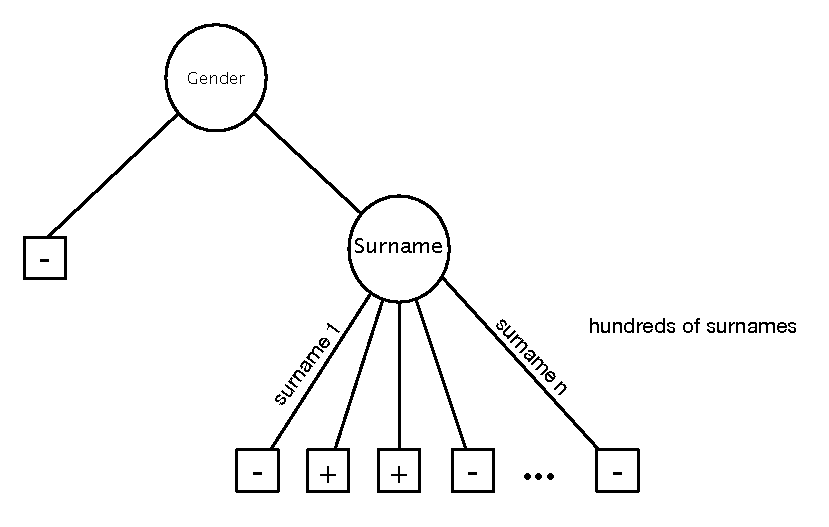
\includegraphics[width=\linewidth]{fig1.pdf}
	\caption{A decision tree for the basic features}
	\label{fig:tree_base}
\end{figure}

The above example showcases that without additional features, an induction algorithm will either overfit its classifier to the given data, or otherwise give a very poor result. Even if we attempt to use standard feature generation approaches, there is no additional information that combinations of these features would find.
However, if we assume that we have access to a relational knowledge base connecting surnames to common countries of origin, we can begin to apply feature generation techniques to the problem, as we can move from the domain of surnames to that of countries. An unsupervised feature generation algorithm might generate a feature for each country of origin, asking whether that surname is common to that country. This would generate dozens of features, most of which are irrelevant to a given example.

Using our approach, we can improve upon this. In the original problem, the node of value female contains objects of type person. Our goal is to separate this set of people to those at high risk and those at low risk. Therefore, Our method defines a new learning problem with the following training set: The objects are surnames; surnames of people with the disease are labelled as positive. The features for these objects are extracted from the knowledge base.
Solving the above learning problem through an induction algorithm yields a classifier on surnames. This classifier can be used as a binary feature in the original problem. For example, it can be used as a feature in the node of value female in figure \ref{fig:tree_base}, yielding the tree seen in figure \ref{fig:lvl1_tree}. 

This new feature gives us a better generalization, as we now abstract the long list of surnames to a short list of countries. This result also allows us to capture previously unseen surnames from those countries. However, this is not a sufficient solution, as we have no way of generalizing on previously unseen countries of origin. An immediate advantage of this approach is that rather than generating dozens of features, most of which are irrelevant, we have created a single feature, that is explicitly based on the concept that we are attempting to learn. 


\begin{figure}
	\centering
	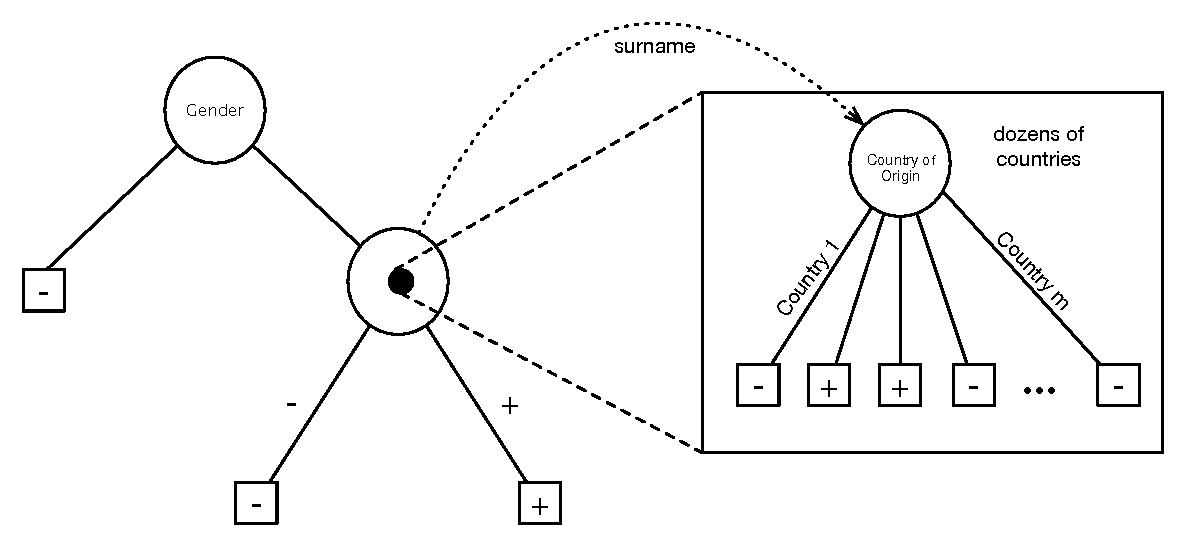
\includegraphics[width=\linewidth]{fig2.pdf}
	\caption{A constructed feature used within a decision tree}
	\label{fig:lvl1_tree}
\end{figure}

Suppose that we also have access to a knowledge base of facts about countries, such as average temperature, precipitation, and more (one such knowledge base is DBpedia). Using such a knowledge base, an unsupervised approach might generate features looking at the properties of the countries that a given surname is common in, giving us features along the lines of ``is this surname common in a country whose population is over 80 million?". Even without thresholding on the values, we would still have many features, most of which are irrelevant to the learning problem at hand.

Following our approach, we can recursively apply our method while trying to learn the new problem. We create a new training set, the objects of which are countries of origin, and countries of surnames of people with the disease are labelled as positive. This training set is given to an induction algorithm using the relational knowledge base about countries to construct features. The result is a classifier that tries to separate between countries of origin of people with the disease and those without the disease. The classifier is used as a feature by the first level recursive algorithm. The whole process is depicted in figure \ref{fig:moving_to_lvl2}. The resulting two-level recursive classifier is depicted in figure \ref{fig:lvl2_tree}. This constructed feature allows us to concisely and accurately capture the target concept, as the construction process is guided by the target concept, in a manner similar to that of deductive approaches.

%We also note that while an unsupervised approach can also create a combination of features that when used together allow us to identify the target concept, the unsupervised nature of the search makes such an attempt computationally expensive, especially when the knowledge base is extensive and multiple logical leaps are necessary.

\begin{figure*}[t]
	\centering
	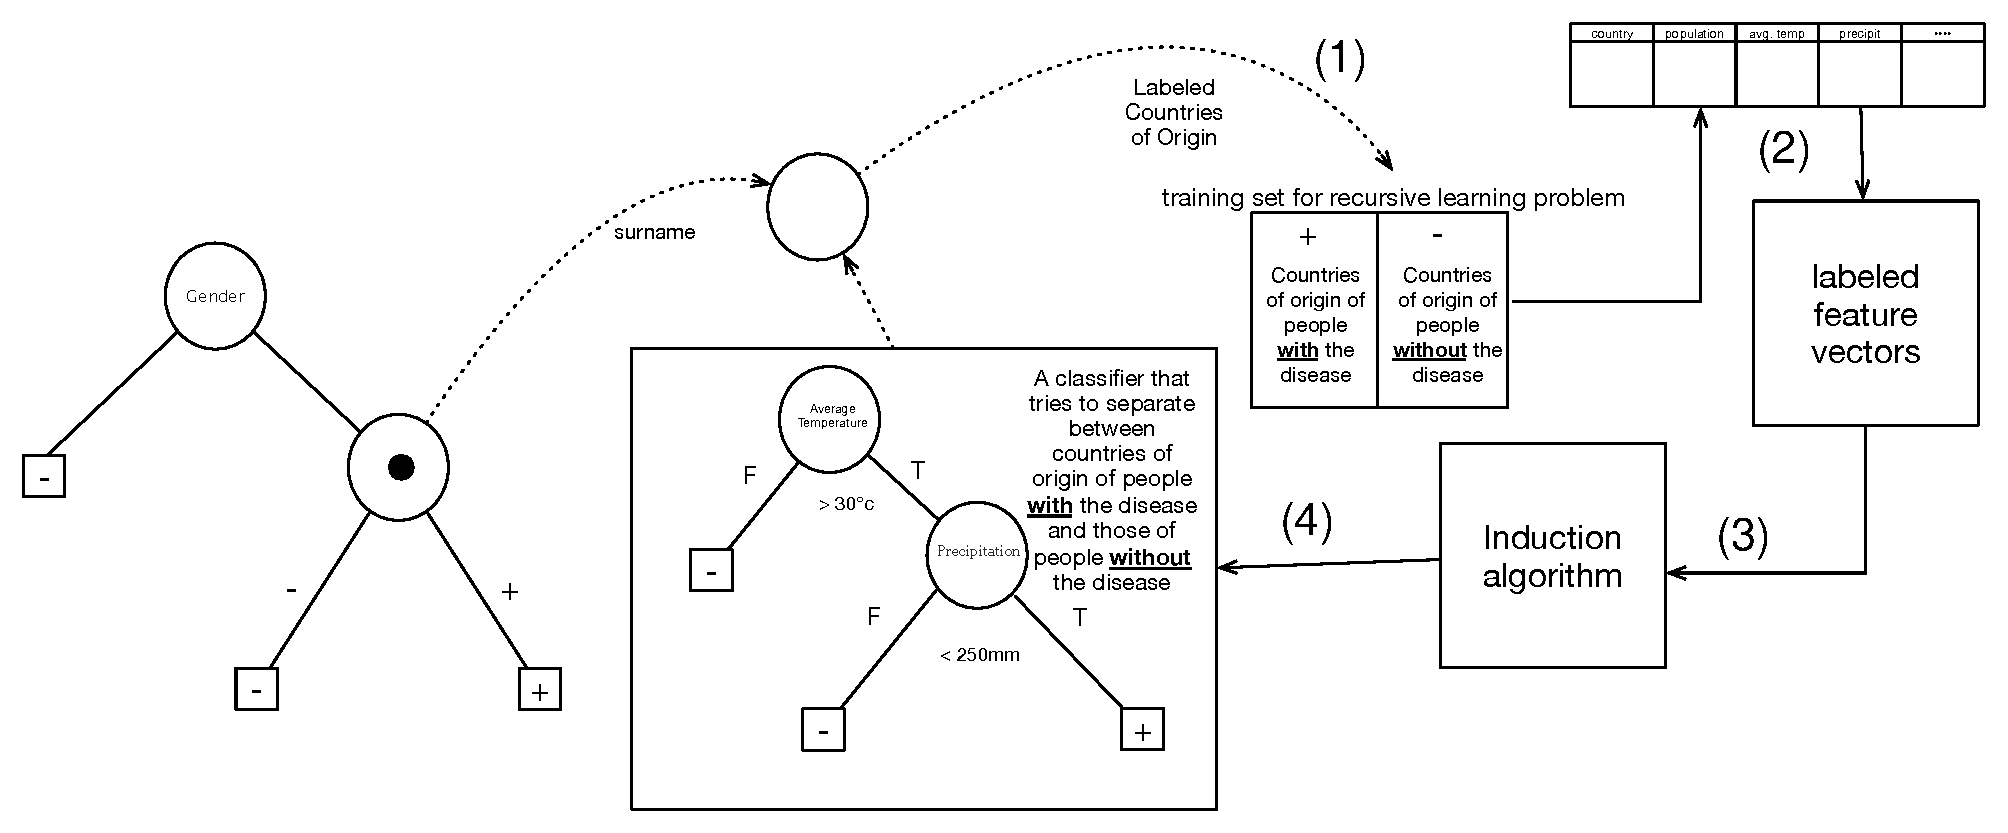
\includegraphics[width=\linewidth]{fig4_annotated.pdf}
	\caption{Recursive construction of a learning problem on countries of origin. $(1)$-Creating the objects for the new problem. $(2)$-Creating features using the knowledge base. $(3)$-Applying an induction algorithm. $(4)$-The resulting feature.}
	\label{fig:moving_to_lvl2}
\end{figure*}

\begin{figure*}[t]
	\centering
	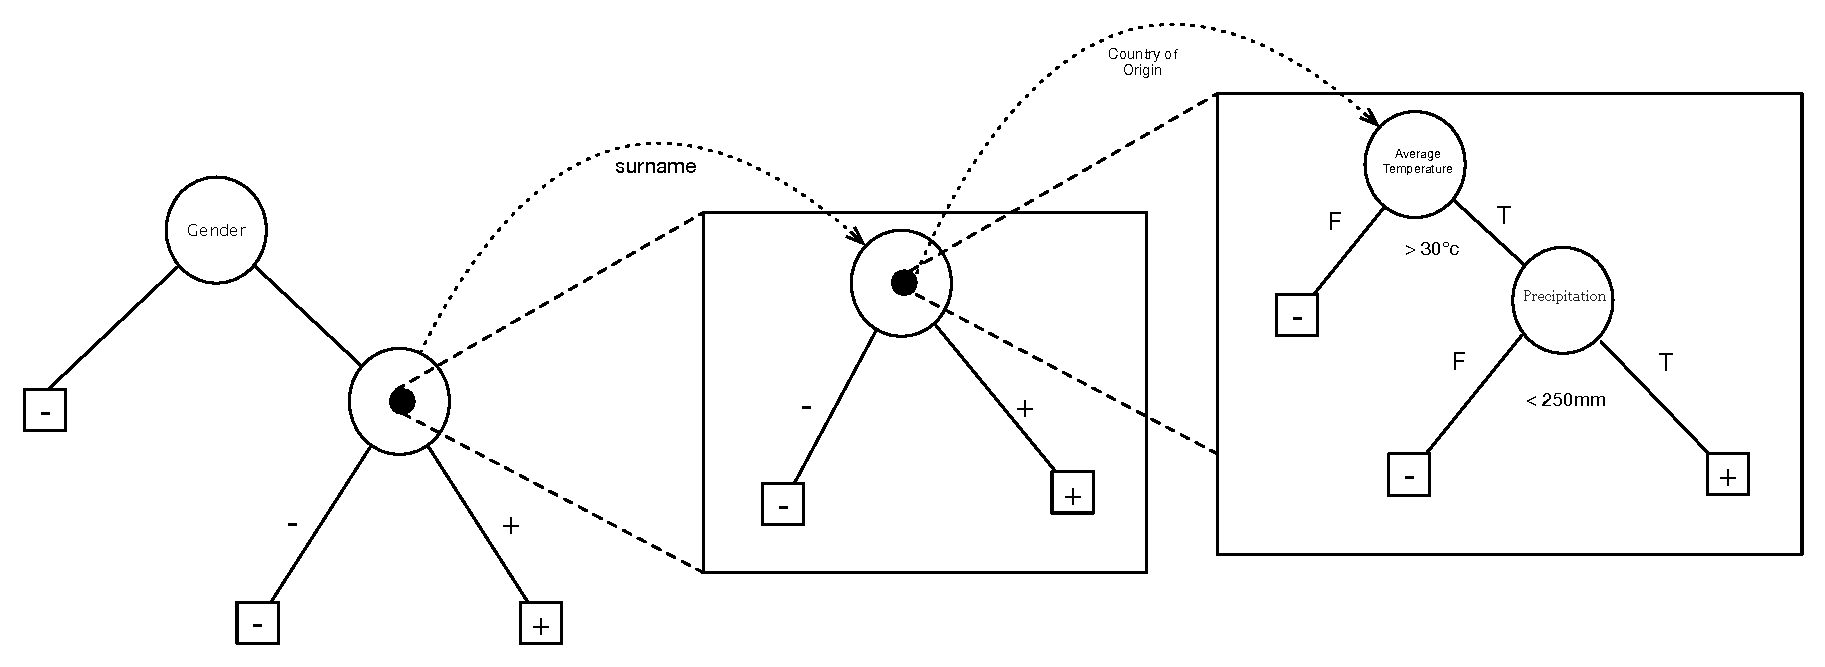
\includegraphics[width=\linewidth]{fig3.pdf}
	\caption{A two-level constructed feature used within a decision tree}
	\label{fig:lvl2_tree}
\end{figure*}

While this is a simple example, it shows a case where additional information and complex features can result in an overall simpler, more general result. It is important to mention that an unsupervised feature generation approach could also solve this problem, but would be forced to generate more features, many of which irrelevant to the problem at hand. In cases where the knowledge base is extensive and contains many connections between entities, complex relationships that are buried deep beneath the surface problem would be computationally expensive to locate, and hard to evaluate once found.


%%%%%%%%%%%%%%%%%%%%%%%%%%%%%%%%%%%%%%%%%%%%%%%%%%%%%%%%%%
%\section{Background} \label{background}
%%%%%%%%%%%%%%%%%%%%%%%%%%%%%%%%%%%%%%%%%%%%%%%%%%%%%%%%%%

%One of the earliest methods of utilizing relational information is \emph{Inductive Logic Programming(ILP)} \citep{quinlan1990learning, muggleton1991inductive}. This approach induces a set of first-order formulae that define a good separation of the given training set.
%Following this work, Relational Learning - techniques designed to utilize relational databases, have become increasingly prevalent. One such technique is that of View Learning \citep{davis2005view}, which generated new tables from existing ones, effectively performing feature generation for relational methods.

%One major attempt at adding relational knowledge to traditional induction algorithms was \emph{propositionalization} \citep{kramer2000bottom}: Since we wish to allow the use of first-order predicates in propositional methods, we create possible (non recursive) first-order predicates in a process known as refinement search \citep{van1998completeness}.
%We define a graph of possible first-order formulae by selecting an initial relation and allowing one of two possible refinement operators: The first operator is binding a single variable in the formula by assigning a constant value to it, and the second is binding a single variable using another relation.

%These operators define a search space. For each formula, we can ask whether a given object satisfies it, giving us a binary query for the data. We often prefer to only use formulae with one unbound variable, as it simplifies the satisfaction check.
%It is important to note that each application of refinement operators yields a formula that is subsumed by the parent, meaning that any object satisfying the child formula will also satisfy its parent.

%A major setback of this process is that it generates an impractically large number of features, most of which irrelevant.  To this end, \emph{upgrade} methods such as ICL \citep{van2001upgrade} were suggested, where instead of creating predicates a-priori, we do so during the training phase, allowing us to avoid searching non-promising refinements.

%As a continuation to this trend, \citet{popescul200716} suggest SGLR, an upgrade method which allows the generation of nominal attributes by using aggregation operators. Essentially, instead of simply checking whether a first-order predicate is satisfied, we perform aggregation over all objects which satisfy it. In addition, SGRL offers an initial insight into the issue of improving the search process by using Akaike's information criteria (AIC, see \citet{burnham2002model}) to select features based on a combination of complexity and predictive power.

%In the case where this external knowledge is organized as a set of relations between entities, several methods can be used. One such method is using \emph{Inductive Logic Programming} \citep{muggleton1991inductive} to generate features, in a process referred to as \emph{upgrading} \citep{van2001upgrade}. This is demonstrated through the ICL algorithm, which uses a refinement graph to search for logical formulae which serve as features. The SGLR algorithm \citep{popescul200716} extends this idea to numerical features, generated using aggregation-based techniques, and then utilizes regression for inference.

%TODO: this section to talk about propo as chain of joins? add that needs serious filtering/subsampling to be tractable, and give newish citations (proposizitonaliztion: wordification blah blah paper?)
%%%%%%%%%%%%%%%%%%%%%%%%%%%%%%%%%%%%%%%%%%%%%%%%%%%%%%%%%%
%\section{Using relational knowledge to generate features: A traditional approach}
%%%%%%%%%%%%%%%%%%%%%%%%%%%%%%%%%%%%%%%%%%%%%%%%%%%%%%%%%%
%Before we discuss our approach, it is prudent to consider existing techniques for turning relational knowledge into additional features.
%Discuss propositionalization?

%%%%%%%%%%%%%%%%%%%%%%%%%%%%%%%%%%%%%%%%%%%%%%%%%%%%%%%%%%
\section{Generating Features through Recursive Induction}
%%%%%%%%%%%%%%%%%%%%%%%%%%%%%%%%%%%%%%%%%%%%%%%%%%%%%%%%%%

We begin our discussion with the standard definition of an induction problem. 
Let $O$ be a set of objects. Let $Y=\{0,1\}$ be a set of labels \footnote{we assume binary labels for ease of discussion}. Let $C:O\rightarrow Y$ be the target concept. Let $S=\{(o_{1},y_{1}),\ldots,(o_{m},y_{m})\}$ be a set of labelled examples such that $o_{i}\in O, y_{i}\in Y, C(o_i)=y_i$. 
Let $F=\{f_{1},\ldots,f_{n}\}$ be a \emph{feature map}, a set of \emph{feature functions} $f_{i}:O\rightarrow Dom_{i}$.  This definition implies a training set represented by feature vectors: $S_F=\{ (\langle f_1(o_i),\ldots,f_n(o_i)\rangle, y_i) | (o_i,y_i) \in S\}$.
Given $S_F$, we wish to find $h_{S_F}:O\rightarrow Y$ such that the generalization error $Sum(o\in O,h_{S_F}(o)\neq C(o))$ is low.

The general task of Feature Generation is as follows: Given $\langle S,F\rangle$, construct a new feature map $F'$ such that when we use an induction algorithm to find a hypothesis, it will generalize more effectively. More formally, $Sum(o\in O,h_{S_F}(o)\neq C(o)) \geq Sum(o\in O,h_{S_F'}(o)\neq C(o))$. Usually, the same induction algorithm is used on both $F$ and $F'$, allowing for a controlled comparison which lowers the impact of the induction algorithm. 

In this work, we assume that in addition to $S_F$ we also have a set of binary \footnote{If our relations are not binary, we can use projection to create multiple binary relations instead} relations ${\cal R}=\{R_{1},\ldots,R_{t}\}, R_j:D_j\times D_{j'}$ representing our knowledge base. 
Intuitively, unless the domains of the knowledge base are relevant for the domains of the feature functions, there is little we can do with this knowledge base. 
Therefore, we add an additional requirement: $\bigcup_{f_i} Dom_i \cap \bigcup_{R_j} D_j \neq \emptyset$. Now that we have formalized the requirements, we can discuss the feature generation problem.

\begin{defn}
	A \emph{supervised feature generation algorithm} based on ${\cal R}$ is an algorithm that given $\langle S,F,{\cal R} \rangle$, creates a new feature map $F_{{\cal R}}=\{f'_{1},\ldots,f'_{l}\}, f'_{k}:O\rightarrow Dom_k$.
\end{defn}

A good supervised feature generation algorithm based on ${\cal R}$ is one that produces lower generalization error during induction. More formally, if given $S_F$, the induction algorithm returns $h_F:O\rightarrow Y$, and given $S_{F_{{\cal R}}}$ the induction algorithm returns $h_{F_{{\cal R}}}:O\rightarrow Y$, a good supervised feature generation algorithm based on ${\cal R}$ must satisfy $Sum(o\in O,h_F(o)\neq C(o)) \geq Sum(o\in O,h_{F_{{\cal R}}}(o)\neq C(o))$.
In order for this to happen, we would like $F_{{\cal R}}$ to be rich enough as to provide us with a better hypothesis, as well as simple and compact enough that such hypothesis can be found with existing induction algorithms.

%We would like the new hypothesis space, defined over $F_{{\cal R}}$, to be one that is both rich enough to provide hypotheses with a lower loss than those in the original space, as well as simple enough that the learning algorithm used will be able to find such good hypotheses given training data.

\subsection{An unsupervised approach to knowledge-based feature generation} \label{shallow_section}

To begin with, we shall try to ignore the labels, and define an unsupervised feature generation algorithm based on ${\cal R}$. We call this algorithm \emph{Shallow}, as it uses the relations in a shallow manner to create features. Using \emph{Shallow}, we can highlight several important concepts.

To begin with, let us first consider the case where all relations are functions, meaning any given relation $R_j$ is a function $R_j:D_j\rightarrow D_{j'}$. In this case, if $Dom_i \subseteq D_j$, we can compose $R_j$ onto $f_i$, giving us a function $f_{i,j}(x)=R_j\circ f_i=R_j(f_i(x)),f_{i,j}:O\rightarrow D_{j'}$. For example, if $f_i$ lists a person's country of origin, and $R_j$ maps countries to their continent, then $f_{i,j}$ lists a person's continent of origin.
Given such $f_{i,j}$, we can either use it as-is, or we can transform it into a set of binary features by specifying the value: $f_{i,j,c}(x)=\begin{cases} 1 &\mbox{if } R_j(f_i(x))=c\\ 
0 & \mbox{otherwise } \end{cases}$ $,f_{i,j,c}:O\rightarrow Y$. In the example above, we might create a feature asking whether a person's continent of origin is Europe.

While this is sufficient in cases where all relations are full functions, in reality knowledge bases are rarely complete, resulting in relations which are partial functions. We shall use $\perp$ to notate \emph{undefined}. A given relation $R_j$ is a partial function $R_j:D_j\rightarrow D_{j'}\cup\{\perp\}$. For example, $R_j$ might map a disease to its preferred treatment method. Sadly, not all diseases are treatable, and thus we have only a partial function.
In this case, $f_{i,j}:O\rightarrow D_{j'}\cup\{\perp\}$ is also a partial function.
During classification, we can then treat $\perp$ as an additional value, allowing us to make use of additional knowledge when it is available. If we wish to have binary features, we must decide whether to treat this value as the condition being unfulfilled, yielding a value of zero, or to exclude it, leading to partial features. We can also treat it as a third possible value, leading to a function $f_{i,j,c}:O\rightarrow Y\cup\{\perp\}$.

Although there are many relations which are also functions, such a requirement may serve as a limitation. For example, a relation mapping a surnames to their countries of origin, as in section \ref{motivation}, may have multiple countries of origin for a single surname. Similarly, a relation mapping a parent to their children may have many children with the same parent.
In cases such as this, $f_{i,j}$ is a set of values, requiring an aggregation function to be used. There are many possible aggregation functions that we can apply on our value set, but we shall discuss three major ones:
\begin{itemize}
	\item All- Given a set of values, whether they all fulfil a certain predicate.
	\item Exists- Given a set of values, whether there exists a value that fulfils a certain predicate.
	\item Majority- Given a set of values, whether a majority of them fulfil a certain predicate.
\end{itemize}
All of the above require a predicate function $p:D_{j'}\rightarrow \{0,1\}$. In the case of $f_{i,j,c}$, that predicate would be $p(x)=c$, and thus using the ``Exists" aggregation function would result in a similar feature, as we would have $f_{i,j,c}(x)=\begin{cases} 1 &\mbox{if } c\in R_j(f_i(x))\\ 
0 & \mbox{otherwise } \end{cases}$.

Now that we have considered all possibilities for the behaviour of a given relation $R_j$ \footnote{Of course, it is possible for a non-function relation to have missing entries. In that case we can easily combine the solutions for both cases.}, we can proceed to define \emph{Shallow}. Given a feature $f_i$, \emph{Shallow} will go over the relations within the knowledge base and attempt to create binary features $f_{i,j,c}:O\rightarrow \{0,1\}$ through the above solutions. \emph{Shallow} then gathers all generated features and outputs them. The pseudo-code is given below.

% Given a feature $f_i$, we take all values of $f_i(x), x\in S$ and see if we can apply relations to them. We then take the resulting values in the relational domain and use them to construct simple binary features of the form $f_{r,c}(x)=\begin{cases} 1 &\mbox{if } \exists f_i\in F :r(f_i(x))=c\\ 
%0 & \mbox{otherwise } \end{cases}$. For example, given a feature that lists a patient's symptoms, we can choose the relation $r=$``Severity" with the constant $c=$``Life-threatening", yielding a feature that will be 1 if and only if a patient is displaying a life-threatening medical issue.

\begin{algorithm}[H]
	\caption{Shallow: Non-recursive Feature Generation using relations}
	\label{code-compete}
	\small
	%insert param stuff
	\begin{algorithmic}
		\Function{CreateFeatures}{$S$,$F$, ${\cal R}$}
		\State $F_{result}=\emptyset$
		\For {$f_i \in F$}
		\For {$R_j \in {\cal R}$ \textbf{where} $Dom_i\cap D_j\neq \emptyset$}
		\State $C=\bigcup_{x\in S} R_j(f_i(x))$ \Comment Constants for $R_j$ with regards to $S, f_i$
		\State  $F_{result}=F_{result}\cup \{f_{i,j,c}(x)|c\in C\}$ \Comment See definition of $f_{i,j,c}:O\rightarrow \{0,1,\perp\}$ above.
		\EndFor
		\EndFor
		\State \Return $F_{result}$ 
		\EndFunction
		
	\end{algorithmic}
\end{algorithm}

We see that this approach allows us to generate features from our knowledge base, regardless of its structure. One example of such features is that of semantic type, features making use of the ``IS-A" relation to note the entity type. We note that this approach create a potentially large number of binary (missing values are treated as zeros) features. While this approach does allow us a degree of generalization, it can only utilize our knowledge base shallowly, from base entities to their values. 
Should we try to apply a chain of relations rather than a single one, even ignoring the many possible scenarios, we must consider the exponential nature of such a chain. Without any way to guide our search through the knowledge base, we are likely to generate and increasingly large number of relations, many of which will be irrelevant. Clearly, if we wish to locate more complex relationships and concepts, a different approach is necessary.

\subsection{Creating Learning Problems using Relations} \label{algorithm_section} 

Now that we have seen how an unsupervised algorithm would make use of a knowledge base for feature generation, we may begin to properly discuss our approach. To do so, we must understand how our approach creates new induction problems using the knowledge base.

Given an original feature $f_{i}:O\rightarrow Dom_i$, our algorithm will formulate a new learning task trying to separate values in $Dom_i$ appearing in positive examples of the original learning task from those appearing in negative ones.  The result of the new learning task will be a classifier
$h_{i}:Dom_{i}\rightarrow Y$ that can label feature values of $f_{i}$. We can then define a new feature $f'_{i}(x)=h_{i}(f_{i}(x)), f'_{i}:O\rightarrow Y$.
We name this algorithm \emph{FEAGURE} (FEAture Generation Using REcursive induction). The full pseudo-code is described in algorithm \ref{code-creating-prob}.

In order to explain how we create such $h_{i}$, let us first consider the creation of a new learning problem. Once we have done so, we can use any induction algorithm to create $h_i$. 
Given a feature $f_{i}$, we first define $v_i(S) = \{v | (o,y) \in S, f_{i}(o)=v\}$ the set of feature values for $f_i$ in $S$. In the intro example, for instance, $v_i(S)$ will b
e the set of all last names of patients that appeared in the training set.
We use $v_i(S)$ as our objects. To define a learning problem, we must consider their labels. 

In the simple case, every feature value appears only for a single example in $S$. In that case, we can simply take the same label, with the result being $label(v)=y$ where $f_i(x)=v,(x,y)\in S$.
Most features in general, and in machine learning task in particular, however, do not have a unique value for each example. In such cases we would have multiple examples in $S$ such that $f_i(x)=v$. Let us call $S(v)$ the set of such examples. In order for us to give a label for $v$, we must aggregate the labels somehow. As in section \ref{shallow_section}, we can consider three major aggregation functions.
Using the All aggregation function results in a strict labelling, as a value will be classified as belonging to the target concept only if all examples in which that value has appeared are labelled positive. The result is consistent label: $label(v)=\begin{cases} 1 &\mbox{if } \forall (x,y)\in S(v): y=1\\ 
0 & \mbox{otherwise } \end{cases}$.
 A more lenient label function is the majority label, taking the Majority aggregation function: $label(v)=majority(\{y|(x,y)\in S(v)\})$.
 
We now formulate a new learning problem with the new training set
$S'_i = \{ (v, label(v)) | v \in v_i(S) \}$.
To fully define our learning problem, we must specify a feature map over $v_i(S)\subseteq Dom_i$. Consider a relation $R_j$ such that $D_j\cap v_i(S)\neq \emptyset$. For such $R_j$, if it is a function, we can simply use it as a feature function, or restrict by a constant $\left(f_{j,c}(v)=\begin{cases} 1 &\mbox{if } \ R_j(v)=c\\ 
0 & \mbox{otherwise } \end{cases}\right)$. If $R_j$ is a partial function, we simply have a feature with missing values. Finally, if $R_j$ is not a function, we can use aggregation as in section \ref{shallow_section} to create features.

Once we have considered all relations in ${\cal R}$, we can generate a feature map for $S'_i$. Given $R_j$, assuming it is relevant to the problem domain, meaning $v_i(S)\cap D_j\neq\emptyset$, we can utilize it as a feature. We then look at all constants $c\in \{R_j(v)|v\in v_i(S)\land R_j(v)\neq \perp\}$. For each such $c$, we add $f_{j,c}:Dom_i\rightarrow \{0,1,\perp\}$ to our feature map. The result of this process is a feature map for $S'_i$, $F_{\cal R}$ which includes all such $f_{j,c}$. We now have a complete induction problem for which we can train a classifier, giving us $h_i:Dom_i\rightarrow Y$. We can then use this $h_i$ on objects in $S$ as discussed above, giving us $f'_{i}(x)=h_{i}(f_{i}(x)), f'_{i}:O\rightarrow Y$. 

We note that once we have an induction problem over $Dom_i$, we can apply our approach recursively on $S'_i$ in order to create additional features. We can see an example of this in section \ref{motivation}, wherein we construct a second-level problem on countries of origin to correctly identify the appropriate conditions that signify high risk countries.
 For each relation $R_j$, rather than restricting it via constants, we take all values of it, and treat those as a feature $f_j(v)=\{v'|R_j(v)=v' \lor v'\in R_j(v) \}$. Assuming $R_j$ is a function or partial function, $f_j$ will also be a function or partial function respectively, and we can then construct a learning problem over values $f_j$, yielding $h_j:D_{j'}\rightarrow Y$. 
 
 In cases where $R_j$ is a relation, $f_j(v)$ is a set of values, essentially a relation as well. In such cases, We must discuss both how to extract a new learning problem, and how a classifier is then used for a set of features.
 To begin with, let us tackle the issue of constructing a learning problem where each feature value is a set. %TODO

\begin{algorithm}[H]
	\caption{FEAGURE-FEAture Generation Using REcursive  induction}
	\label{code-creating-prob}
	\small
		%insert param stuff
		\begin{algorithmic}
			\Function{ConstructFeatures}{$F$, $S$, ${\cal R}$}
				\For {$f_i\in F$}
				\State $S'_i,F_{new}$= \Call{CreateNewProblem}{$f_i$,$S$,${\cal R}$} \Comment{We can apply our algorithm recursively here}
				\State $h_i$= \Call{InductionAlgorithm}{$S'_i,F_{new}$} 
				\If {\Call{Compare}{$h_i,F$}$\geq0$} 
				\State add $h_i$ to new features
				\EndIf
				\EndFor
				\State \Return new features
			\EndFunction
			\State 
			\Function{CreateNewProblem}{$f_{i}$, $S$, ${\cal R}$}
                \State $v_i(S) = \{v | (o,y) \in S, f_{i}(o)=v\}$
                \State $S'_i = \{ (v, label(v)) | v \in v_i(S) \}$ 
                \Comment $label(v)$ can be, for example, the majority function.
                \State $R(v_i,{\cal R}) = \left\{ r \in {\cal R} | v_i(S) \subseteq \{x_1 | (x_1,x_2) \in r\}\right\}$
                \State $F_{new}=\{r(v)=c| c\in Range(r), r\in R(v_i,{\cal R})\}$
                \State \Comment These are features from $Dom_{i}$ to $\{0,1\}$.
                \State \Return $S'_i, F_{new}$ 
                \Comment Our new training set and features define a learning problem.
			\EndFunction
			
		\end{algorithmic}
	\end{algorithm}

We note that while this algorithm deterministically defines a learning problem for a single feature $f_i$, we can use a variety of known machine learning techniques to create $h_i$.
This approach also allows us to apply a comparison between existing features 

%\subsection{Creating Multiple Features} \label{multi_feature}

%Now that we have discussed how we create a single feature, we must consider how to expand this and generate multiple features. One simple approach would be to simply apply the above technique (algorithm \ref{code-creating-prob}) once for each feature.
%Naturally, this would result in $n$ new features.
%Even if we apply the above approach recursively, we would still obtain only $n$ new features, though they may be stronger as we have generated new features within each learning problem.
%Thus, if we wish to generate a larger number of features, we must take a different approach.

%While most traditional machine learning algorithms yield useful properties such as filtering and regularization, a Decision Tree classifier offers several useful traits with regards to recursive application of our approach:
%\begin{enumerate}
%	\item Decomposability: A Decision Tree classifier can be easily decomposed into multiple Decision Stumps, allowing us to decide between generating a single strong feature or multiple weaker features.
%	\item Interpertability: Decision trees are generally considered easier to interpret and understand, allowing us to easily grasp which relations are more impactful, and thus which domains are likely to contain additional knowledge which we may not have utilized.
%	\item Orthogonality: Since features further down in a decision tree are orthogonal to ones already used, we can effectively limit our search space, as relations we have already used will not be picked. This also has a beneficial side effect of increasing variety in generated features.
%\end{enumerate}

\subsection{Finding Locally Improving Features} \label{tree_usage}

When performing feature generation, we often wish to evaluate the predictive power of generated features. When such evaluation is done in the context of the entire dataset, it is possible to lose the unique benefit of a potentially powerful feature. To address this phenomenon, we decided to apply our recursive feature generation algorithm in a divide-and-conquer approach through the use of a Decision Tree, thus allowing us to better identify features with a strong local impact.

While most traditional machine learning algorithms yield useful properties such as filtering and regularization, a Decision Tree classifier offers several useful traits with regards to recursive application of our approach:
\begin{enumerate}
	\item Decomposability: A Decision Tree classifier can be easily decomposed into multiple Decision Stumps, allowing us to decide between generating a single strong feature or multiple weaker features.
	\item Interpertability: Decision trees are generally considered easier to interpret and understand, allowing us to easily grasp which relations are more impactful, and thus which domains are likely to contain additional knowledge which we may not have utilized.
	\item Orthogonality: Since features further down in a decision tree are orthogonal to ones already used, we can effectively limit our search space, as relations we have already used will not be picked. This also has a beneficial side effect of increasing variety in generated features.
\end{enumerate}
It is important to note that the features generated in this process can be later used for \emph{any} induction algorithm.

First, we construct a decision tree node, go over the feature set $F$ and evaluate as normal. We then apply algorithm \ref{code-creating-prob} on all features in $F$, creating our new recursive features. Now, we compare between new and existing features, and pick the best one. We used Information Gain Ratio \cite{quinlan1986} for that comparison.  
Next, we create son nodes based on feature values, and apply the process recursively until we reach a depth/node size limit in order to avoid over-fitting. 
Finally, the features generated during the decision tree training procedure are collected and returned for use as general, black-box features which can be used along with any induction algorithm. The decision tree itself is discarded.


\begin{algorithm}[H]
	\caption{Deep FEAGURE-Decision Tree Feature Generation}
	\label{code-tree-thing}
	\small
		minSize- minimal size of a node in the decision tree.

        SplitByFeature- a method that splits a training set according to a feature.
        
		\begin{algorithmic}
			\Function{ConstructFeaturesInANode}{$S$, $F$, ${\cal R}$}
                \If {$|S|<$minSize} 
                    \State
                    \Return \Call{SplitByFeature}{$S$, f}, $\emptyset$
                \EndIf
                \State newFeatures=\Call{FEAGURE}{$S$, $F$, ${\cal R}$}
                \State $f_{best}$=\Call{bestFeature}{$S$,$F\cup$ newFeatures}
                \State \Return \Call{SplitByFeature}{$S$, $f_{best}$}, newFeatures
			\EndFunction

            			
			\State 
            \Function{ConstructFeatures}{$S$, $F$, ${\cal R}$}
                \State currentFeatures= $\emptyset$
                \State sons, $F_{new}$=\Call{ConstructFeaturesInANode}{$S$, $F$, ${\cal R}$}
                \State currentFeatures= currentFeatures$\cup F_{new}$
                \For {son in sons}
                    \State newFeatures=\Call{ConstructFeatures}{son.$S$,$F$,${\cal R}$}
                    \State currentFeatures= currentFeatures$\cup$newFeatures
                \EndFor
                \State \Return currentFeatures
			\EndFunction
		\end{algorithmic}
	\end{algorithm}

%%%%%%%%%%%%%%%%%%%%%%%%%%%%%%%%%%%%%%%%%%%%%%%%%%%%%%%%%%
\section{Applications for Text Categorization}
%%%%%%%%%%%%%%%%%%%%%%%%%%%%%%%%%%%%%%%%%%%%%%%%%%%%%%%%%%

The text Categorization problem is defined by a set of texts $X$ labelled by a set of categories $Y$ such that we create $S=\{(x_i,y_i)|x_i\in X, y_i\in Y\}$. Given $S$, The learning problem is to create a hypothesis $h:X\rightarrow Y$ which minimizes error (mistaken label).
The standard approach to solving this problem is based on the bag-of-words \cite{Wu:1981:CST:1013228.511759,salton1983introduction} approach, Using the frequencies of word appearances within the text as features and thus learn $h$.

As discussed, we have seen the recent rise of Semantic Linked Data as a powerful knowledge base for text-based entities, with large databases such as Google Knowledge Graph \cite{pelikanova2014google}, Wikidata \cite{vrandevcic2014wikidata} and YAGO2 \cite{hoffart2013yago2}. Naturally, we would like to make use of such semantic data to improve upon the bag-of-words approach, with the implicit assumption that additional Semantic knowledge will allow us to better approximate the relationship between the text and its given label.

Since semantic data utilizes entities, not words and texts as its underlying knowledge components, we must apply some approach which extracts entities from texts. There is a multitude of such methods, such as Named Entity Recognition (NER),  Wikification \cite{bunescu2006using} and Entity Linking \cite{rao2013entity}.
Using the above approaches, we can convert a text $x$ into a set of entities $e(x)$.

\subsection{FEAGURE for Text Categorization}

Given a set of texts converted to entities, we can define $f_i(x)=E(x)$ the entities within the text. We then define ${\cal R}$ to be the set of relations within our knowledge base. Combining these definitions with algorithm \ref{code-creating-prob} we get $v_i(S)=\cup_{x_i}{E(x_i)}$ the set of entities for all texts, $R(v_i,{\cal R})$ is the set of relations in our knowledge base that apply to all entities, and $F_{new}$ would be a set of functions mapping entity keys to their values with regards to relation $r$, so $f_r(x)=\{c|\exists e\in E(x):r(e)=c\}$.

We notice two important difference from the general case that must be discussed.
Firstly, the suggested scheme only considers relations that apply to all entities contained within the text. While such relations exist (for example, the IS-A relation which describes entity type), most relations within a standard knowledge base do not apply to all entity types. To combat this, we allow the use of relations that apply only to some entities (based on domains), allowing us to use all relations within the knowledge base. However, as a result of this it is possible that $f_r(x)=\emptyset$, which will, in turn, mean that the resulting $h$ created during feature generation will be inapplicable to $x$. As a result, $h$ is a partial function $h:X\rightarrow \{0,1\}$, and when using FEAGURE we will have three child nodes: One for value $1$, one for value $0$, and a third for value inapplicable.

The second major difference we must consider is the possibility of having multiple entities for which the resulting classifier applies, potentially yielding multiple classifications for $x$ \footnote{For example, a text mentioning multiple countries, each classified differently by $h$}. To best resolve this, in cases where a feature is applicable to multiple unique words within the text, we return a majority vote of the classification returned by the feature as applied to each such word, as seen in figure \ref{figure5}

\begin{figure}[t]
	\centering
	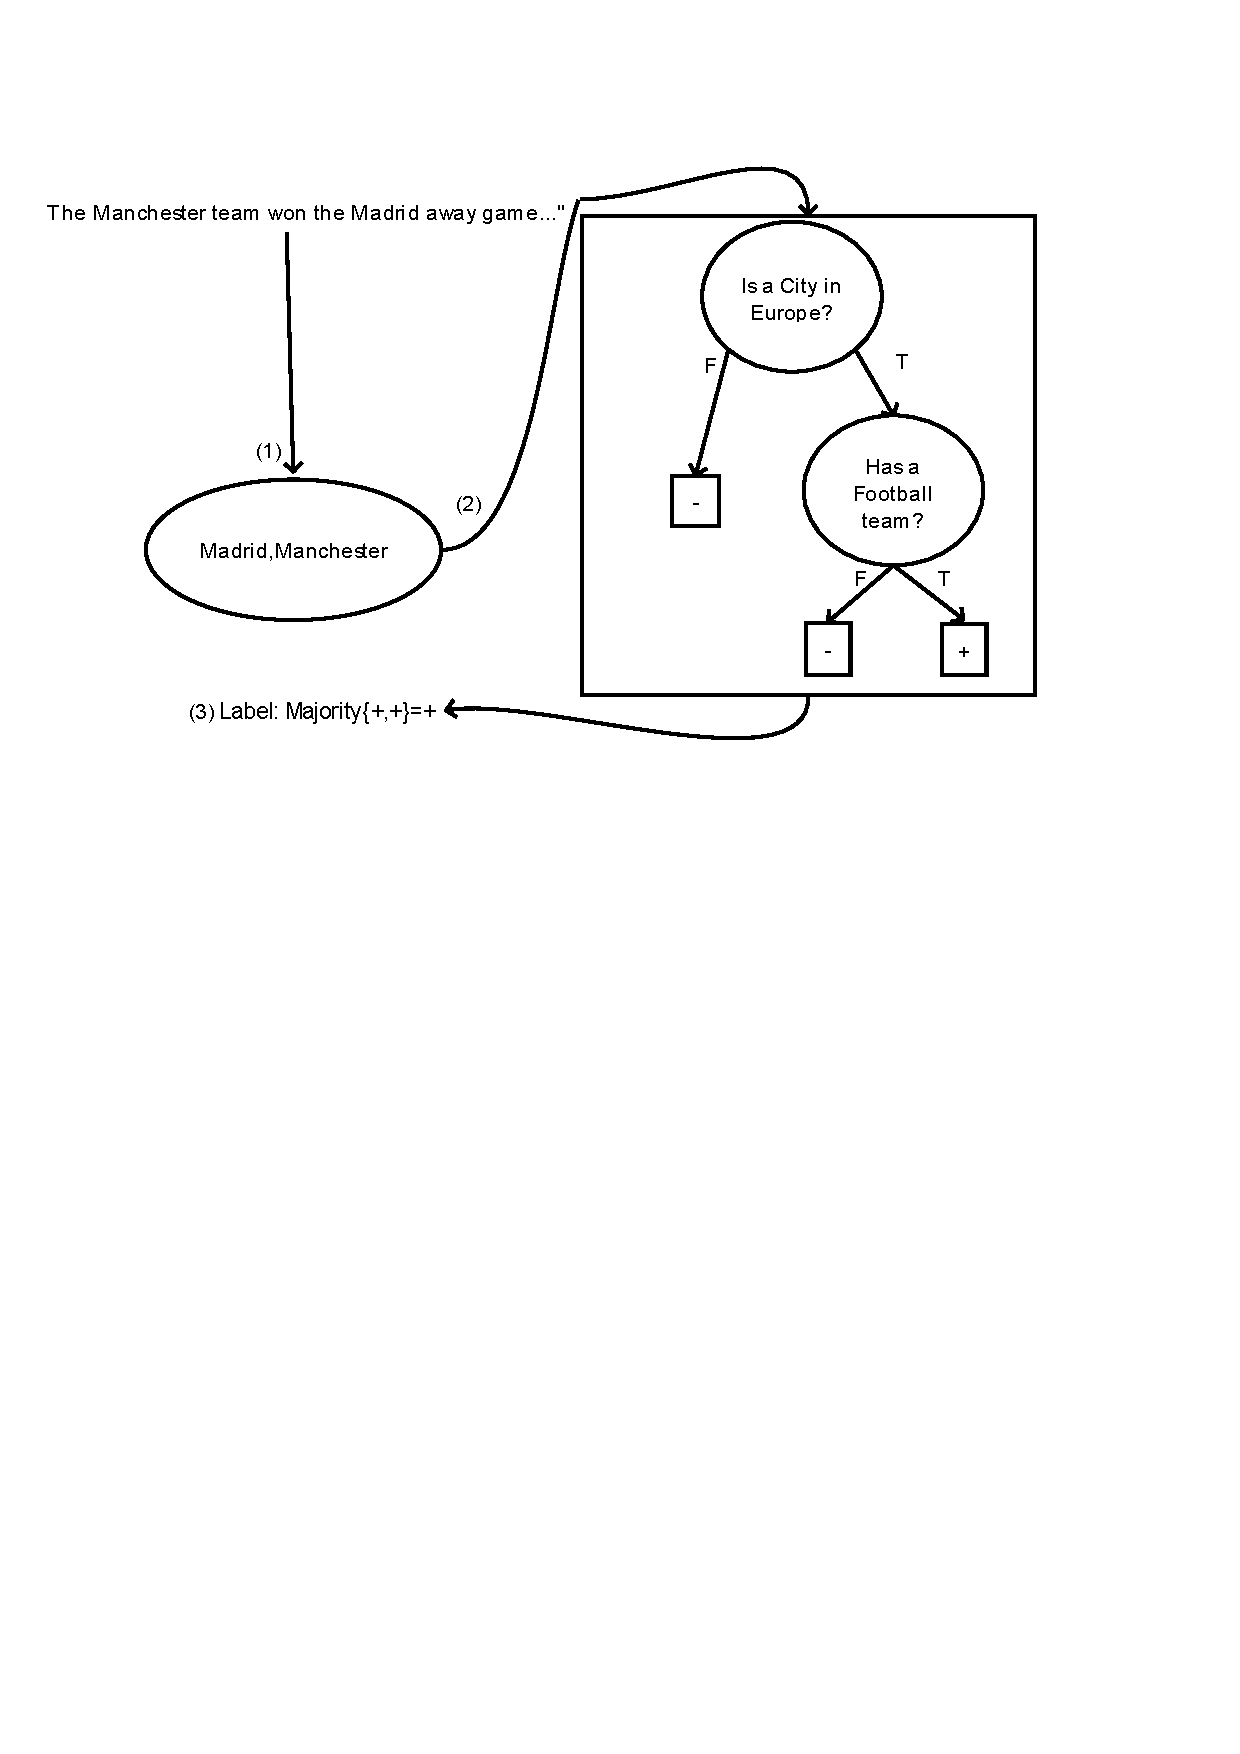
\includegraphics[width=\linewidth]{fig5.pdf}
	\caption{Using a constructed feature in text: $(1)$-Relevant entities are extracted. $(2)$-Each entity is sent to the constructed feature. $(3)$-A majority vote between responses is performed.}
	\label{figure5}
\end{figure}

%%%%%%%%%%%%%%%%%%%%%%%%%%%%%%%%%%%%%%%%%%%%%%%%%%%%%%%%%%
%\section{Discussion and Analysis of the FEAGURE algorithm}
%%%%%%%%%%%%%%%%%%%%%%%%%%%%%%%%%%%%%%%%%%%%%%%%%%%%%%%%%%

%tree in outer allows looking at 1 feature a time->more structured search

%We note that in order to prevent cycles which provide no new information, we do not allow the use of any relation that is the inverse of a previously used relation.

%The process of re-labelling and constructing recursive problems as detailed in section \ref{algorithm_section} offers some unique contributions:
%\begin{itemize}
%	\item By moving our domain space when constructing a new problem, we essentially look at the problem from another perspective, which allows for the discovery of complex relationships.
%	\item The process of re-labeling allows noise reduction and emphasizes more general trends within the data that may be harder to otherwise notice.
%	\item We can exploit the power of existing, well-developed learning algorithms when we create a classifier, and possibly use different ones as we take recursive steps.
%\end{itemize}
%Furthermore, we note that FEAGURE can locate locally useful features which may be difficult to identify when looking at the dataset as a whole.

%The resulting features of the FEAGURE algorithm %TODO: discuss that they are classifiers on feature values. also talk on the fact that we expect a few powerful&complex features, rather than many simple ones

%In terms of runtime performance, while FEAGURE has a large overhead, we note two major things: Firstly, the critical section of re-labeling and constructing recursive problems can be parallelized for different recursive problems within a decision tree node.
%Secondly, we note that existing approaches such as the ones described by  \citeA{cheng2011automatedfull} and \citeA{paulheim2012unsupervisedfull}, as well as propositionalization approaches %TODO: citations. possibly this is mentioned earlier?
%perform a chain of join operations ($\Join$) between existing feature values and external knowledge bases, which require similar overheads in terms of performance.

%%%%%%%%%%%%%%%%%%%%%%%%%%%%%%%%%%%%%%%%%%%%%%%%%%%%%%%%%%
\section{Empirical Evaluation}
%%%%%%%%%%%%%%%%%%%%%%%%%%%%%%%%%%%%%%%%%%%%%%%%%%%%%%%%%%
In this section, we discuss our experimental methodology and display our main results.

\subsection{Metodology}

In order to evaluate a Feature Generation algorithm, we first activate it on the training set of an existing learning problem in order to generate new features. Once we have generated our new feature set, we proceed to test it by learning a classifier on the training set and measuring its accuracy against a testing set. We made use of two well-known learning algorithms for this task: SVM \cite{cortes1995support} and K-NN \cite{fix1951discriminatory}\footnote{For SVM we used a linear kernel and a regularization parameter $C=10$; for K-NN we used $K=3$}.

\subsubsection{Datasets}

For evaluation, we used two datasets:
\begin{enumerate}
	\item \textbf{TechTC-100} \cite{gabrilovich2004text} - A collection of 100 different binary text categorization problems of varying difficulty, extracted from the Open Dictionary project. On each dataset, we used the Stanford Named Entity Recognizer \cite{finkel2005incorporatingfull} for entity recognition. We then performed stopword elimination using NLTK \cite{bird2009natural} and performed stemming using the Porter Stemmer \cite{van1980new}.
	We evaluated our results by measuring accuracy based on the training and testing sets defined in the original paper. Additionally, we tested our feature set both without feature selection, as well as with a $5\%$ feature selection, which as \citeA{gabrilovich2004textresults} demonstrated, yielded good accuracy.
	
	As our knowledge base, we used \textbf{YAGO2} \cite{hoffart2013yago2}, omitting any relations with literal data such as dates or geographic coordinates. For each relation within YAGO2, we created both the relation itself as well as the inverse relation, and then removed reverse relations that map very few values to very many \footnote{For example, the inverse of the ``has gender" relation  maps ``male" and ``female" to all to all existing people within the YAGO2 database.}. YAGO2 contains approximately 2 million entities and 124 million facts.
	
	This dataset collection served as a powerful benchmark, as it contains small multiple text classification problems of varying difficulties. We used YAGO2 as our knowledge base as it contains a great deal of general knowledge - facts regarding countries, events and individuals.
	\item \textbf{OHSUMED} \cite{hersh1994ohsumed} - A dataset of medical abstracts from the MeSH categories of the year 1991. Similarly to \citeA{joachims1998text}, we use only the first 20,000 documents. Furthermore, we limit ourselves to medical documents that contain only a title (that is, there is no available abstract). On each document, stopword elimination and simple stemming was used (due to the medical nature of the texts, the porter stemmer performed poorly). For entity extraction, we used Wikipedia Miner \cite{milne2013open}.  In addition, we only take two categories, C1 and C20 \footnote{Bacterial Infections and Mycoses, Immunologic Diseases} as a binary learning problem. We then applied ten-fold cross validation on the resulting document set to rigorously test  our approach.
	
	As our knowledge base, we used \textbf{Freebase} data dump used by \citeA{bast2014easy}, taking only entities relevant to our domain. This smaller dump of the Freebase knowledge base contains approximately 49 million entities and 242 million facts regarding multiple domains. Data regarding the medical domain is far more sparse, containing roughly a hundred thousand facts in total.
	
	This dataset served as a test case representing a larger, more specialized learning problem, where domain-specific knowledge is required. Thus, Freebase, which contains a large body of medical knowledge, was more suitable. 
\end{enumerate}

\subsubsection{Experiment Parameters}

We tested the following parameters:
\begin{enumerate}
	\item Recursion level: We ran our feature generation algorithm for both a depth of one, creating a recursive learning problem for the original problem, and a depth of two, creating recursive learning problems within a generated learning problem. 
	\item Tree depth: As discussed in section \ref{tree_usage}, we use Deep-FEAGURE within a decision tree. In order to avoid over-fitting, we limit both tree depth and node size, proportionately to the size of the training set. We experimented with the parameter of maximal tree depth to test its effect on the accuracy of the resulting features.
	\item Induction algorithm: In section \ref{algorithm_section}, we define FEAGURE without specifying the induction algorithm used to generate features within the new learning problem. We ran most of our experiments using a decision tree induction algorithm for that purpose. We also experimented with using other induction algorithms, namely SVM and K-NN.
	\item Feature Filtering technique: In section \ref{algorithm_section}, we use a generic function comparing constructed features with existing ones in order to filter constructed features. We experimented with both a feature based on maximal Information Gain (IG) and one based on average IG, both taking into account all baseline non-relational features.
\end{enumerate}


 %We also limit these parameters accordingly within the generated recursive problems, as they also utilize a decision tree as their classifier. To decide whether a tree classifier was sufficiently beneficial, we compared its information gain ratio (including the value of inapplicable) to the information gain ratio of the feature with highest information gain ratio. We then allowed a $50\%$ negative penalty parameter to encourage picking generated features assuming they were better than $50\%$ times the best information gain for that decision tree node. 

%For labelling objects within constructed learning problems, we use the majority label - The label of an object within the constructed problem will be the label corresponding to the majority of texts containing the entity that was the relation key. Similarly, we use the majority label when deciding on the output of the constructed classifier- In cases where our classifier outputs multiple labels for a single text, we simply take the label corresponding to the majority. We can see an example of this in figure \ref{figure5}.






%%%%%%%%%%%%%%%%%%%%%%%%%%%%%%%%%%%
\subsection{Main Results}
%%%%%%%%%%%%%%%%%%%%%%%%%%%%%%%%%%%

Table \ref{table:acc} shows average accuracies across all 10 folds for OHSUMED, as well as the average accuracies for datasets in techTC-100. Statistical significance over baseline is shown in parenthesis. Best results are marked in bold.
For the TechTC-100 dataset, we see a significant improvement over the baseline and shallow approaches, even though fewer features are generated than the competing algorithm. We also see that for SVM, the two-level application gives poorer results than the single level FEAGURE algorithm. This can be attributed to over-fitting effects resulting from a combination of mistakes in entity extraction as well as the small dataset size. Due to the nature of linear SVM, such a feature will have significant impact on performance.

Analysis of the results for the OHSUMED datasets show that for K-NN, we do not achieve an improvement over the baseline approach (and neither does shallow). For SVM, we see a significant improvement over the baseline approach, with a single level application achieving a $3.2\%$ increase in accuracy, and a two-level application giving a total of $2.4\%$ improvement.

\begin{table}[]
	\centering
	\caption{Average number of generated features for each dataset, using FEAGURE, a 2-level activation of FEAGURE, and the Shallow algorithm. }
	\label{table:features}
	\begin{tabular}{|l||l|l|l|}
		\hline
		& \# Features(FEAGURE)  & \# Features(FEAGURE 2-level)  & \# Features(Shallow) \\ \hline
		OHSUMED      & 506.2           & 732        & 27162.2                \\ \hline
		TechTC-100  & 63.3       & 65.06      & 5004.66 \\ 
		\hline             
	\end{tabular}
\end{table}

\begin{table}[]
	\centering
	\caption{Average accuracy. The columns specify feature generation approach, with baseline being no feature generation. The rows specify the induction algorithm used on the generated features for evaluation. TechTC-100 has an additional entry for 5\% feature selection, meaning only 5\% of all features (maximal IG) are used.}
	\label{table:acc}
	\begin{tabular}{|l | l || l | l | l| l|}
		\hline
		Dataset & Classifier & Baseline   & Shallow & FEAGURE   & FEAGURE 2-level    \\ \hline
		\multirow{2}{*}{OHSUMED} & KNN  & 0.766 & \textbf{0.766} & 0.761   & 0.744 \\ \cline{2-6}
		& SVM  & 0.789 & 0.789   & \textbf{0.814 ($p<0.01$)}    & 0.808 \\ \specialrule{.15em}{.05em}{.01em} % \hline
		
		\multirow{2}{*}{TechTC-100} & KNN & 0.526 & 0.526 & 0.533 ($p<.05$) & \textbf{0.552 ($p<.001$)}  \\ \cline{2-6}
		& SVM  & 0.694 & 0.694   & \textbf{0.712 ($p<0.001$)}    & 0.691 \\ \specialrule{.15em}{.05em}{.01em}
		
		\multirow{2}{*}{TechTC-100 (5\%)} & KNN  & 0.613 & 0.592 & \textbf{0.629 ($p<0.001$)}   & 0.619 \\ \cline{2-6}
		
		& SVM  & 0.693 & 0.692   & \textbf{0.707 ($p<.001$)} & 0.704 ($p<0.05$) \\ \hline
		 
	\end{tabular}
\end{table}

%results for svm, results for knn, discuss differences and compete-alg.
Before we look at varying parameters of our algorithm, let us analyze the results on TechTC-100 to better understand the impact of our approach on datasets of varying difficulty. Figure \ref{fig:svm_base_lvl1} shows the accuracies for datasets in techTC-100 using a SVM classifier, The x axis represents the baseline accuracy without feature generation, and the y axis represents the accuracy using our new feature set using FEAGURE. Therefore, any dataset that falls above the $y=x$ line is an improvement in accuracy. We use this visualization technique to illustrate our results on the techTC-100 dataset collection.

\begin{figure}
	\centering
	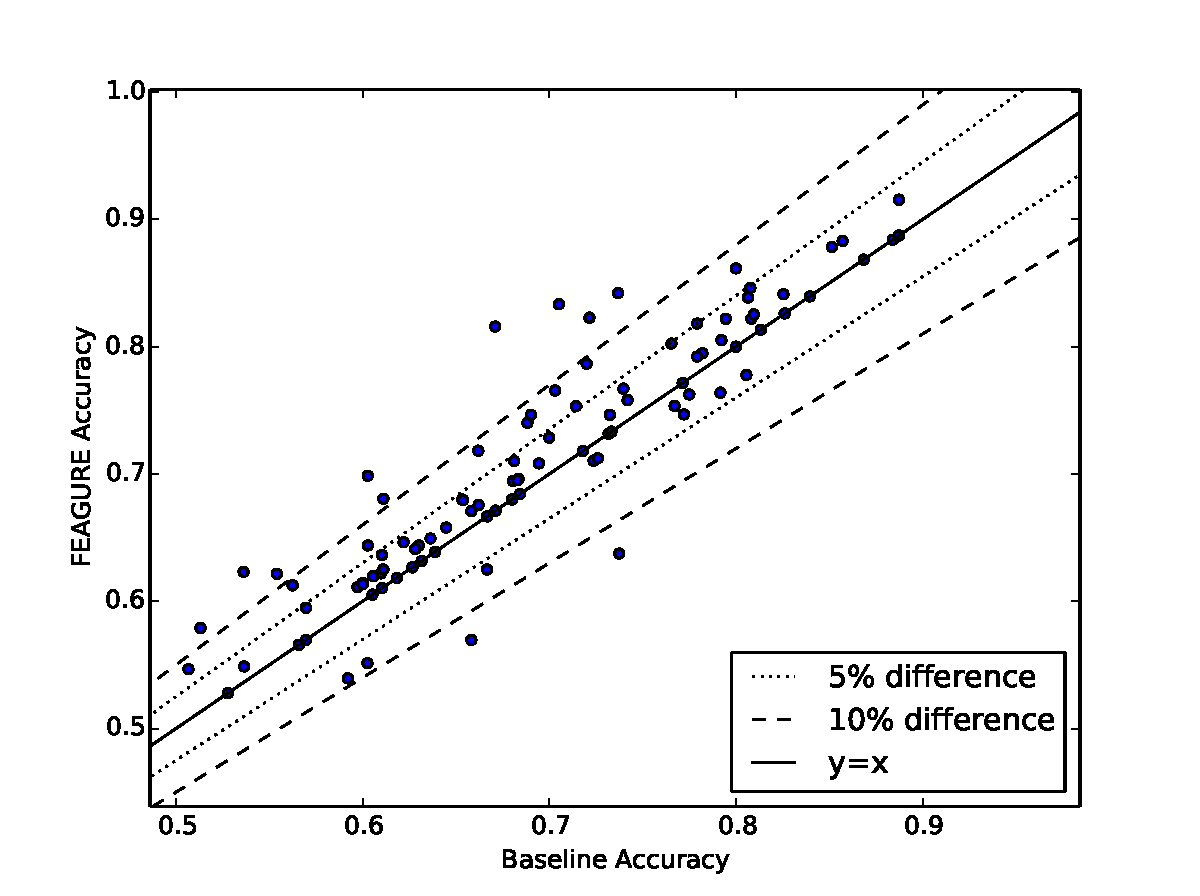
\includegraphics[width=0.8\linewidth]{new_svm_10_base_vs_lvl1}
	\caption{Accuracy of
		baseline approach compared to single activation of FEAGURE (SVM). Each point represents a dataset. The dotted lines represent a 5 and 10 percent difference in accuracy}
	\label{fig:svm_base_lvl1}
\end{figure}

The results for show a general trend of improvement, with high ($> 5\%$) or very high ($>10\%$) improvement being common. We also see multiple datasets where no features are generated, with few datasets showing a degrade in accuracy.
This can be attributed to two major causes:
\begin{itemize}
	\item Errors in the entity extraction process may lead to the creation of misleading entities and thus features. For instance, the word ``One" may be interpreted as the entity ``One (Metallica song)". 
	\item Over-fitting within the feature generation algorithm may create features that appear to have high information gain while generalizing poorly to test data.
\end{itemize}

Figure \ref{fig:25best} shows the 25 hardest datasets in TechTC-100, in terms of the Maximal Achievable Accuracy (MAA) criterion defined by  \citeA{gabrilovich2004text}. We see that for most of these, we achieve improvement, with a $5\%$ or higher increase being common. We also see several datasets where no features are generated (and thus the accuracy is the same) and a single dataset that shows a minor degrade in accuracy. This results illustrates that we can, in general, rely on FEAGURE to yield positive recursive features on difficult classification problems.

\begin{figure}
	\centering
	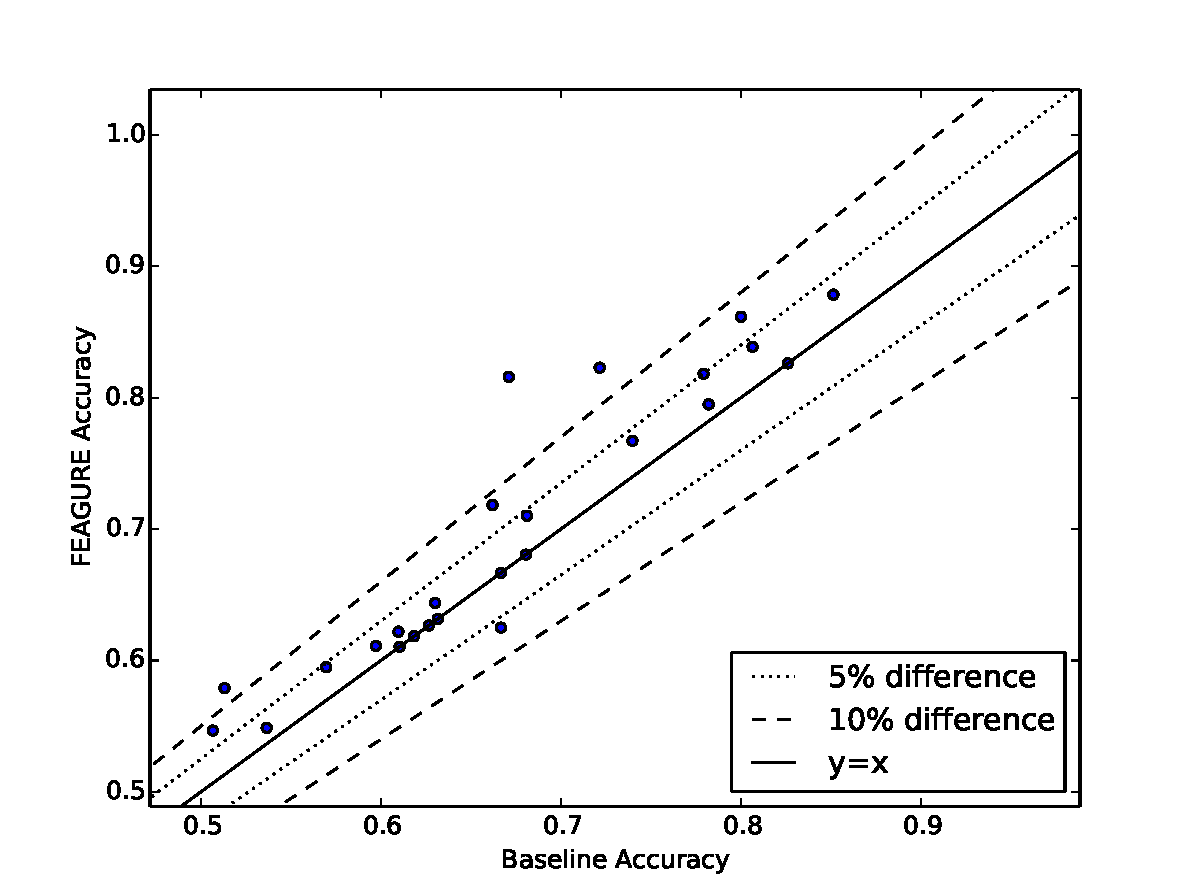
\includegraphics[width=0.8\linewidth]{new_svm_10_25hardest}
	\caption{Accuracy of
		baseline approach compared to single activation of FEAGURE (SVM). 25 Hardest datasets (lowest minimal accuracy)}
	\label{fig:25best}
\end{figure}

\subsection{Using Non-Tree classifiers with FEAGURE}

As we have discussed in section \ref{algorithm_section}, algorithm \ref{code-creating-prob} creates a generic learning problem as part of its execution. In this section, we will test the effects of using various induction algorithms on these recursive problems. We have chosen to try both K-NN and SVM, with the following parameters: For K-NN, we used $K=3$. For SVM we used $C=10$, with both Linear and a Radial Basis Function (RBF) kernels.

%Table \ref{table:features-nontree} shows the average number of generated features. We see that these approaches generate far fewer features on average. This should come as no surprise, as we cannot flatten constructed recursive trees in order to generate additional features, nor do we run the learning algorithms on smaller problems.
Table \ref{table:acc-nontree} shows the accuracies achieved by these approaches. We see that while in general, the results are poorer than those achieved by our approach, we do see a clear improvement in accuracy for many of these cases, including the case of K-NN for the OHSUMED dataset.
Looking at the amount of features generated, we see that on average, these approaches generate far fewer features. This should come as no surprise, as the tree-based classifier uses flattening to create additional features.

%\begin{table}[]
%	\centering
%	\caption{Average Number of Generated Features}
%	\label{table:features-nontree}
%	\begin{tabular}{lllll}
%		& \# Features(Tree)  & \# Features(Linear SVM)  & \# Features(RBF SVM) & \# Features(3-NN) \\
%		OHSUMED      & 506.2  &  24.7 & 34.5  & 14.6     \\
%		TechTC-100  & 63.3   &   12.04    &  8.95   & 4.25        
%	\end{tabular}
%\end{table}

\begin{table}[]
	\centering
	\caption{Average accuracy. The columns specify the induction algorithm used in FEAGURE (Decision Tree, SVM with linear or RBF kernel, K-NN). The rows specify the induction algorithm used on the generated features for evaluation. TechTC-100 has an additional entry for 5\% feature selection, meaning only 5\% of all features (maximal IG) are used.}
	\label{table:acc-nontree}
	\centering
	\begin{tabular}{|l | l || l | l| l|l|}
		\hline
		Dataset & Classifier  & Tree-FEAGURE & Linear SVM   & RBF SVM & 3-NN    \\ \hline
		\multirow{2}{*}{OHSUMED} & KNN  & 0.761 & 0.756   & \textbf{0.783} & 0.744 \\ \cline{2-6}
		& SVM   & \textbf{0.814}  & 0.795  & 0.796 & 0.788 \\ \specialrule{.15em}{.05em}{.01em} % \hline
		
		\multirow{2}{*}{TechTC-100} & KNN  & \textbf{0.533} & 0.531 ($p<0.05$) & 0.527 &  0.528 \\ \cline{2-6}
		& SVM    & \textbf{0.712} &  0.705 ($p<0.005$)  & 0.698 ($p<0.05$) & 0.697 \\ \specialrule{.15em}{.05em}{.01em}
		
		\multirow{2}{*}{TechTC-100 (5\%)} & KNN  & \textbf{0.629 ($p<0.001$)}  & 0.625 ($p<0.05$) & 0.61 & 0.617 \\ \cline{2-6}
		
		& SVM   & \textbf{0.707 ($p<.001$)} & 0.697 & 0.7 ($p<0.05$) & 0.699 ($p<0.05$)\\ \hline
		
	\end{tabular}
\end{table}

\subsection{Effect of Feature Filtering on Accuracy}

In this section we look at the effect of using a different evaluation method for generated features. In algorithm \ref{code-tree-thing}, we use a comparison function which compares the constructed feature to the best non-relational feature. It may be the case, however, that we should compare our feature in some way to all existing features. One way to do so is to use the mean Information Gain Ratio of features in $F$. Should our new feature score lower than the average, we filter it out. 

%\begin{table}[]
%	\centering
%	\caption{Average Number of Generated Features}
%	\label{table:features-average}
%	\begin{tabular}{lllll}
%		& FEAGURE  & FEAGURE 2-level  & Average IG &  Average IG 2-level \\
%		OHSUMED      & 506.2           & 732        &    1270.6   &   1371.4       \\
%		TechTC-100  & 63.3       & 65.06      &  234.43 &  244.05             
%	\end{tabular}
%\end{table}

\begin{table}[]
	\centering
	\caption{Average accuracy. The columns specify feature filtering approach, being either the average information gain (IG) or the maximal. The rows specify the induction algorithm used on the generated features for evaluation. TechTC-100 has an additional entry for 5\% feature selection, meaning only 5\% of all features (maximal IG) are used.}
	\label{table:acc-average}
	\begin{tabular}{|l | l || l | l || l| l|}
		\hline
		Dataset & Classifier & Max-IG   & Average-IG & Max-IG 2-level  & Average-IG 2-level    \\ \hline
		\multirow{2}{*}{OHSUMED} & KNN  & \textbf{0.761} & 0.667 & 0.744   & 0.686 \\ \cline{2-6}
		& SVM  & \textbf{0.814} & 0.811   & 0.808    & 0.81 \\ \specialrule{.15em}{.05em}{.01em} % \hline
		
		\multirow{2}{*}{TechTC-100} & KNN & 0.533 & 0.553 ($p<0.001$) & 0.552 & \textbf{0.555 ($p<.001$)}  \\ \cline{2-6}
		& SVM  & 0.712 & \textbf{0.728 ($p<0.001$)}    & 0.691   & 0.653 \\ \specialrule{.15em}{.05em}{.01em}
		
		\multirow{2}{*}{TechTC-100 (5\%)} & KNN  & 0.629 & \textbf{0.646 ($p<0.001$)} & 0.619   & 0.594 \\ \cline{2-6}
		
		& SVM  & 0.707 & \textbf{0.724 ($p<.001$)}   &0.704 & 0.707 ($p<0.05$) \\ \hline
		
	\end{tabular}
\end{table}

%Table \ref{table:features-average} shows the amount of features generated by FEAGURE. We see that the amount is significantly greater, indicating that this is a more lax requirement than the one we used (over half of the best information gain ratio). 
Table \ref{table:acc-average} shows the accuracies attained through this change. For the TechTC-100 dataset collection, we see a general increase in accuracy, especially for single level application. For the OHSUMED dataset, we cannot detect a meaningful improvement, and for K-NN see a degrade in accuracy. 
Looking at he number of features generated reveals that using the average IG yields roughly twice the number of features in tech-TC, and even larger on OHSUMED. 
These results indicate that for small problems, generating additional features is preferable, whereas for problems with many examples, a stronger filtering mechanism is more advantageous. 


\subsection{Effect of Search Tree Depth on Accuracy}

In this section, we test at the usefulness of searching local problems for additional features.
To do so, we run FEAGURE while limiting the depth of the search tree in algorithm \ref{code-tree-thing}. 
We compare our two datasets side-by-side.

\begin{figure}
	\centering
	\begin{subfigure}{.55\textwidth}
		\centering
		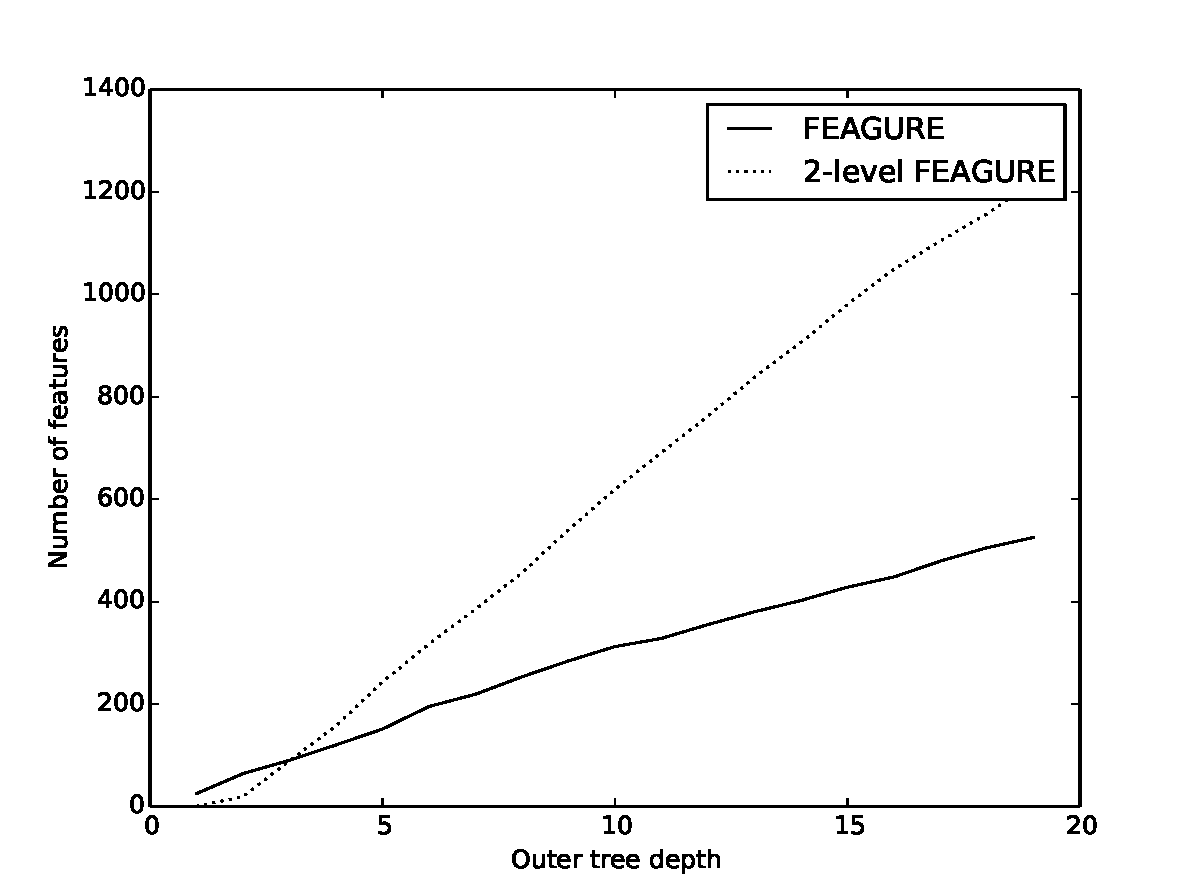
\includegraphics[width=1.1\linewidth]{num_features_ohsumed.pdf}
		\caption{OHSUMED}
		\label{fig:features-depth-ohsumed}
	\end{subfigure}%
	\begin{subfigure}{.55\textwidth}
		\centering
		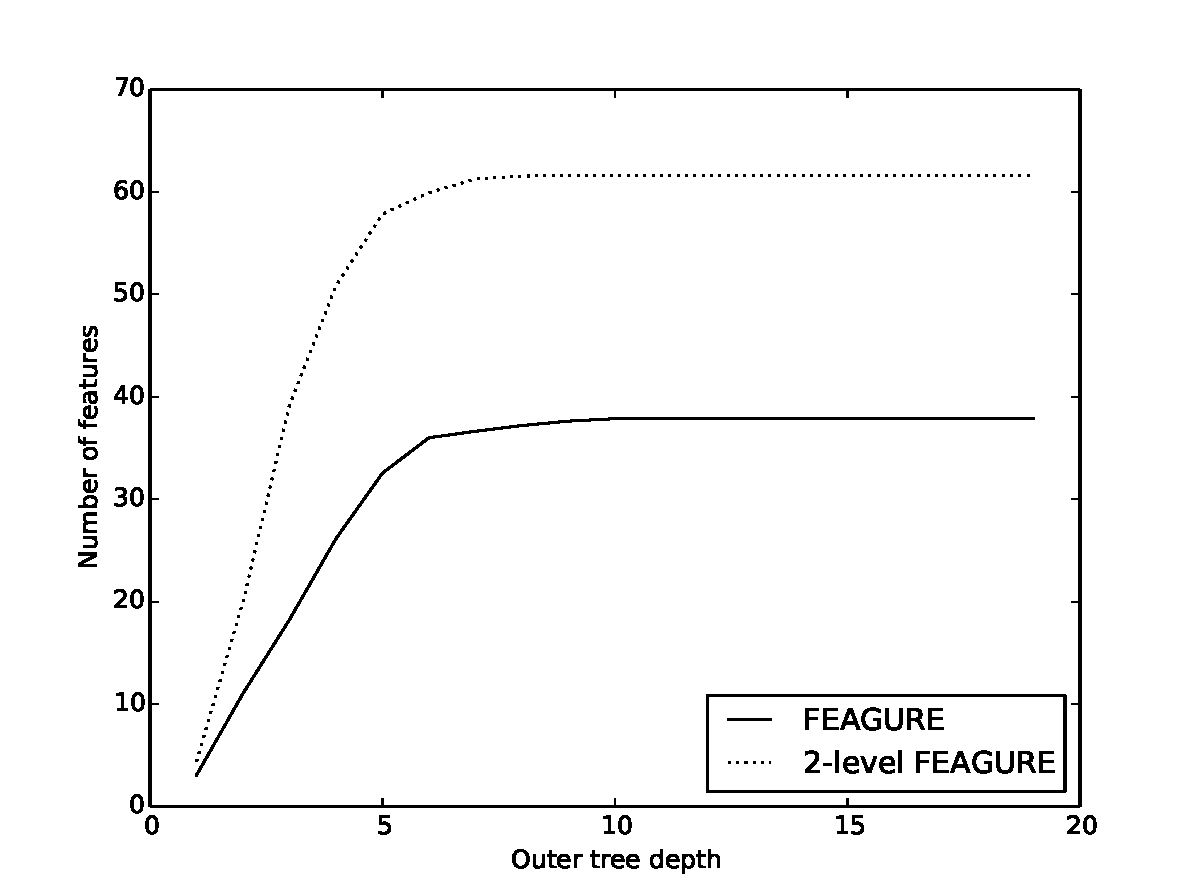
\includegraphics[width=1.1\linewidth]{num_features_techtc.pdf}
		\caption{TechTC-100}
		\label{fig:features-depth-techtc}
	\end{subfigure}
	\caption{Mean number of features generated}
	\label{fig:features-depth}
\end{figure}

Figure \ref{fig:features-depth} shows the number of generated features per depth.  For both datasets, we see a linear increase, with a two-level application showing a faster increase. In TechTC-100, we see that after a certain depth, there is no additional gain. This is due to the small size of the learning problems.

\begin{figure}
	\centering
	\begin{subfigure}{.55\textwidth}
		\centering
		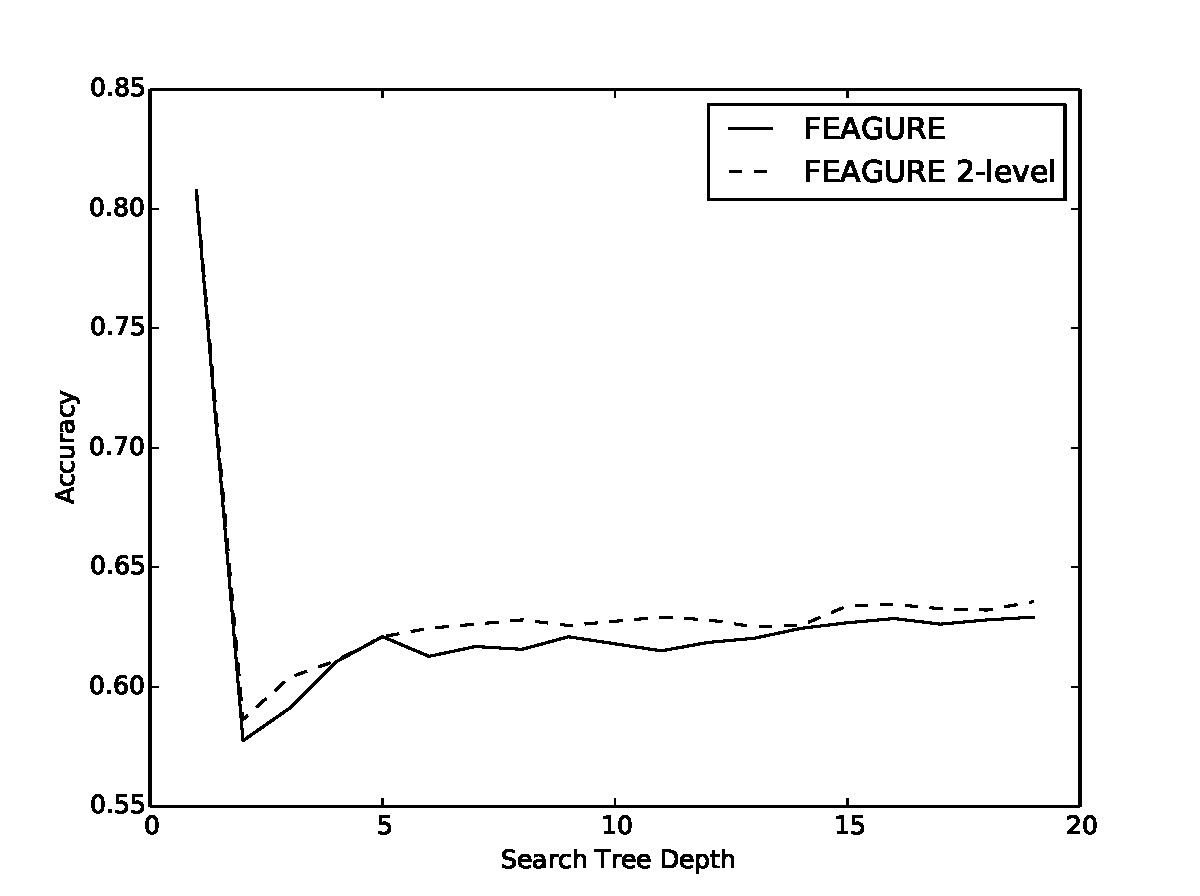
\includegraphics[width=1.1\linewidth]{new_depth_ohsumed.pdf}
		\caption{OHSUMED}
		\label{fig:svm-ohsumed}
	\end{subfigure}%
	\begin{subfigure}{.55\textwidth}
		\centering
		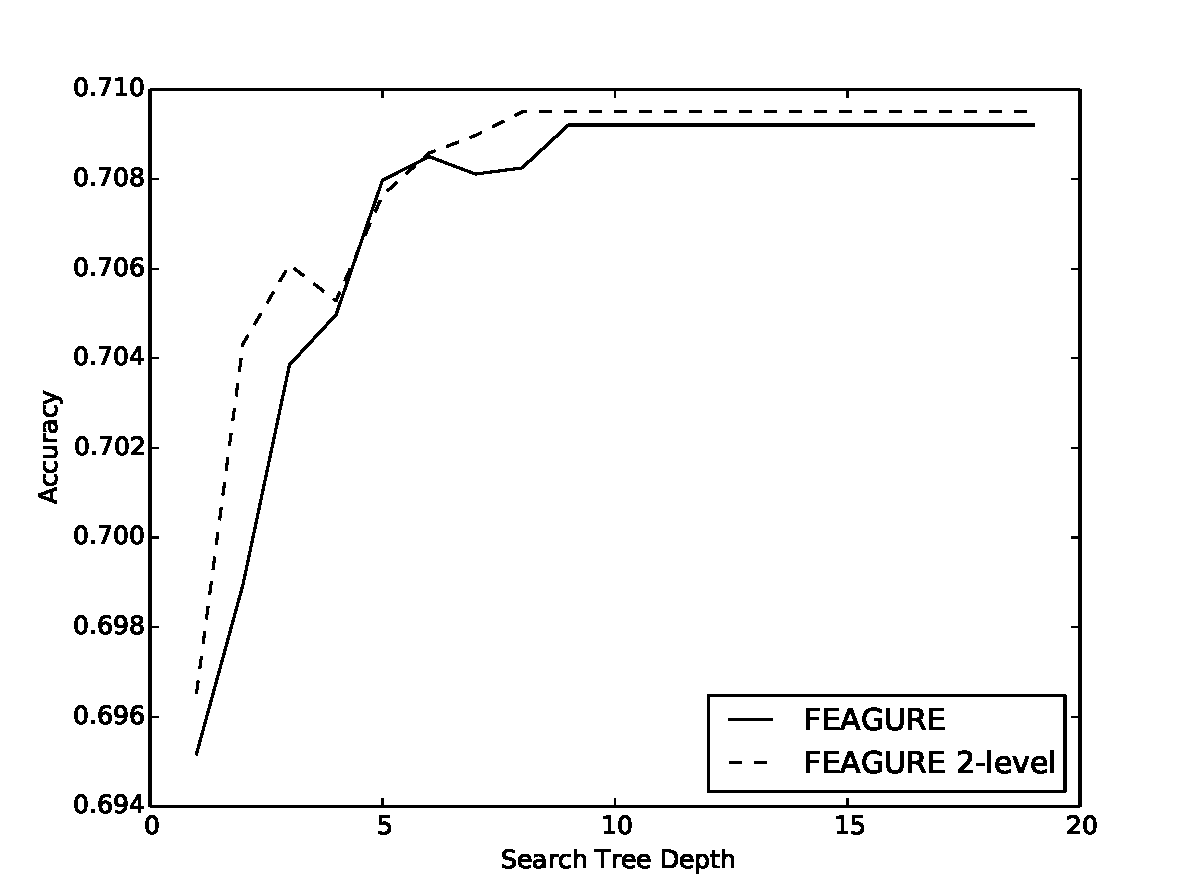
\includegraphics[width=1.1\linewidth]{new_depth_005_techtc.pdf}
		\caption{TechTC-100}
		\label{fig:svm-techtc}
	\end{subfigure}
	\caption{Mean SVM Accuracy}
	\label{fig:svm-acc}
\end{figure}

Figure \ref{fig:svm-acc} shows the mean accuracy of a SVM classifier for increasing depths. The results for K-NN classifiers are similar their general trend. In TechTC-100, we see a trend of increasing accuracy, up to a saturation point. This is to be expected, as adding largely orthogonal features would yield improvement until a maximal depth is achieved.

For OHSUMED, however, we see a sharp fall in accuracy, followed by a recovery. 
This is caused by the orthogonality of features down the tree combined with errors in entity extraction causing features immediately following the first few tree nodes to separate on mistakenly extracted entities.

In both cases, we see that the two level application of Deep-FEAGURE yields slightly better accuracy on average.

%\subsection{Qualitative Analysis}
%In order to better understand the contribution of these features, let us look at several of them to try and better understand them. Figure \ref{fig:level1_good} shows one of the features generated for single level feature generation. We can see that the feature attempts to separate based on geographical location. Figure \ref{fig:level1_simple} shows a simple feature regarding people, and showcases the fact that when there is no need for overly complex features, our technique will not force such features. This feature yields a $10\%-15\%$ increase in accuracy (depending on feature selection level), and is generated by both the single and two level approaches.

%Figure \ref{fig:level2_tree} showcases the additional power of the level two approach. The second level learning problem separates non-countries from countries, as well as countries which deal with non fuel manufacturing Arabic nations from those who embargo them.

%Figure \ref{fig:weird_trees} showcases some of the unique oddities of using our technique with the YAGO2 knowledge base. Since YAGO groups together all entities which have a grammatical gender (including fictional characters and non-living objects) under a single relation, the constructed feature looks at both deceased individuals and words that are the same as Australian television channels (such as Gold and Galaxy) at the same time.

%\begin{figure}[]
%	\centering
%	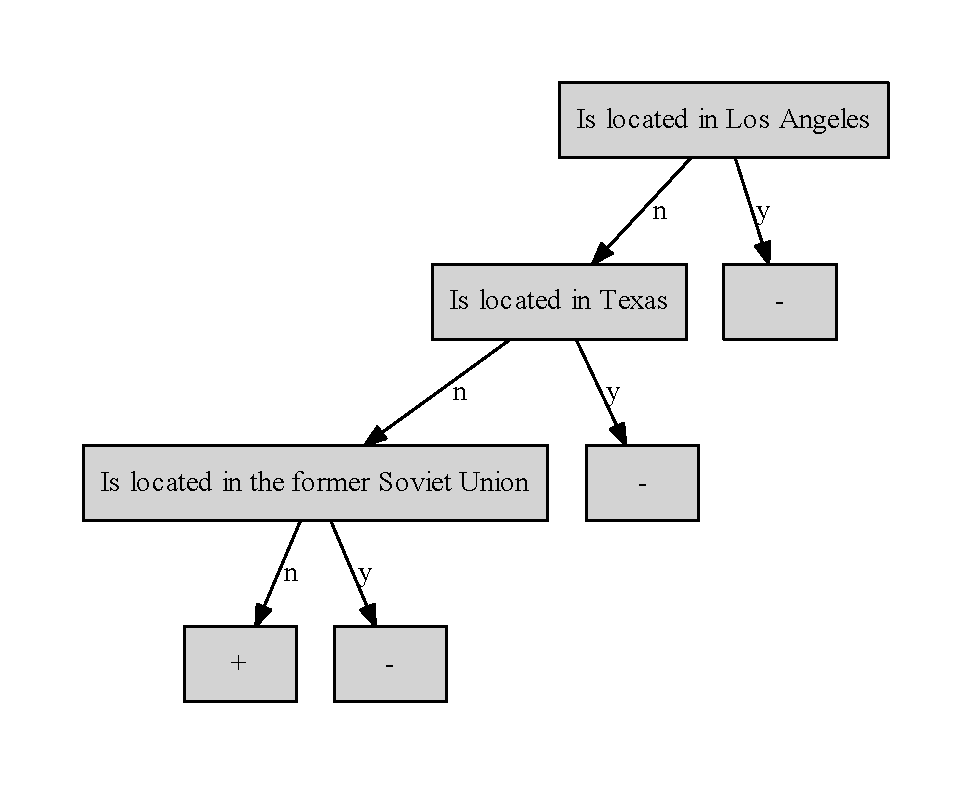
\includegraphics[width=0.8 \linewidth]{level1_good.pdf}
%	\caption{A single level feature regarding nations and organizations with official websites}
%	\label{fig:level1_good}
%\end{figure}

%\begin{figure}[]
%	\centering
%	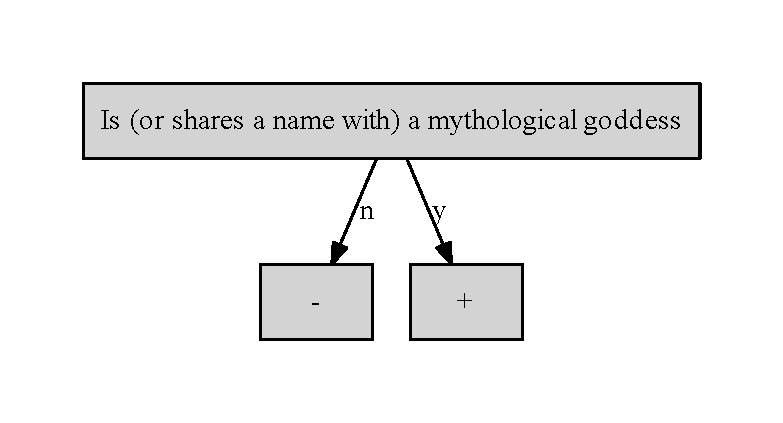
\includegraphics[width=0.6 \linewidth]{level1_simple.pdf}
%	\caption{A single level feature regarding people (real or fictional)}
%	\label{fig:level1_simple}
%\end{figure}

%\begin{figure}[]
%	\centering
%	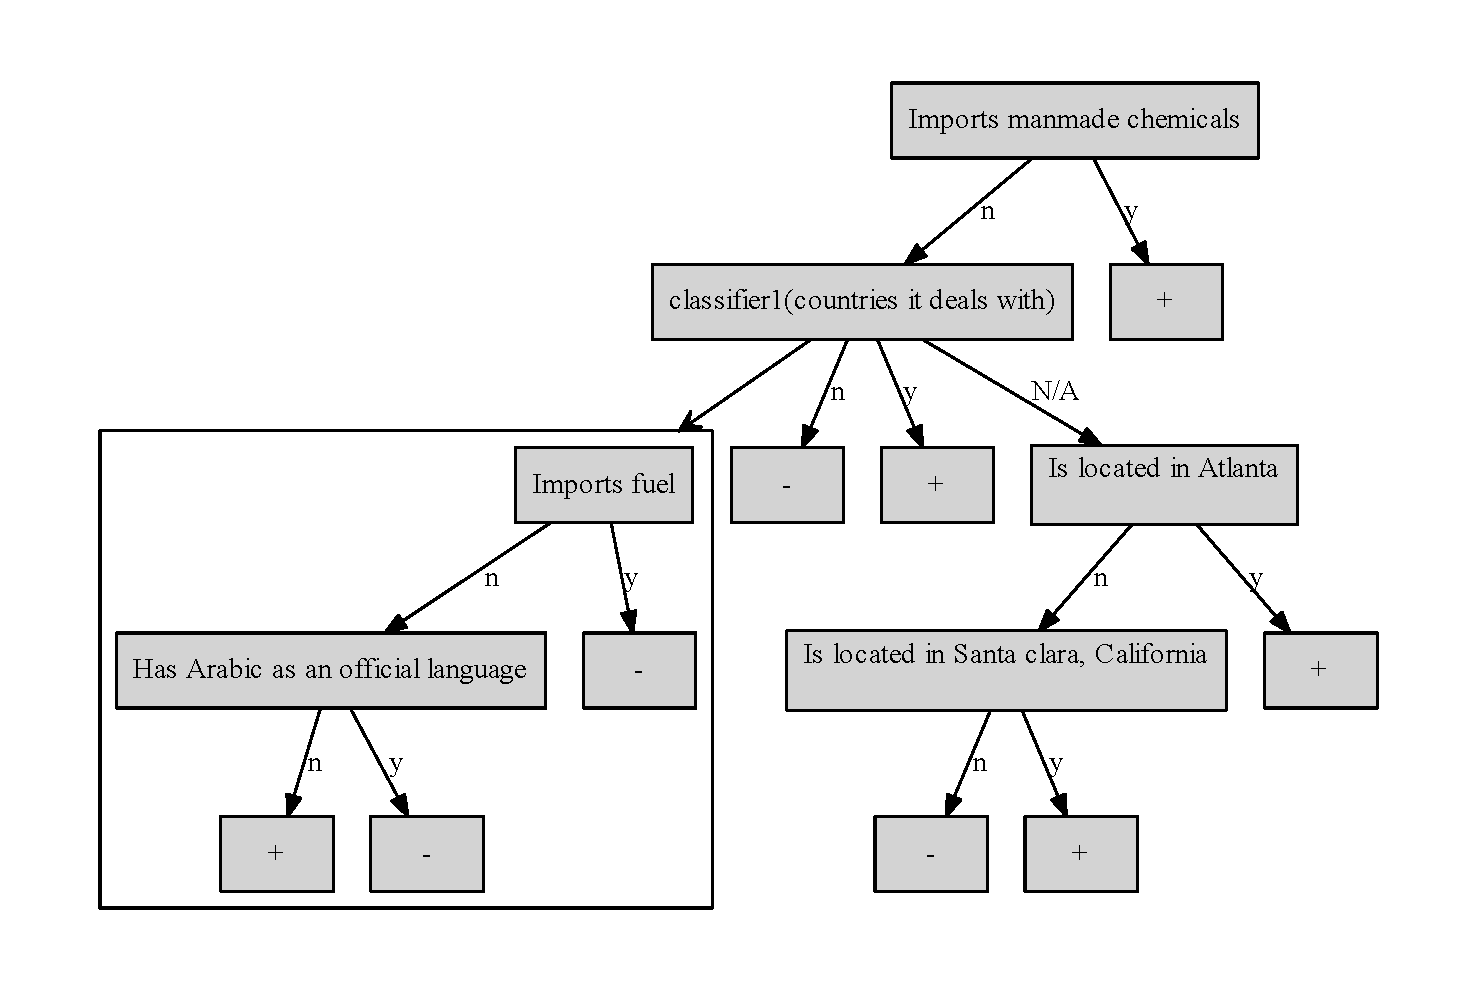
\includegraphics[width=\linewidth]{level2_tree.pdf}
%	\caption{A two level feature regarding countries and organizations}
%	\label{fig:level2_tree}
%\end{figure}

%\begin{figure}[]
%	\centering
%	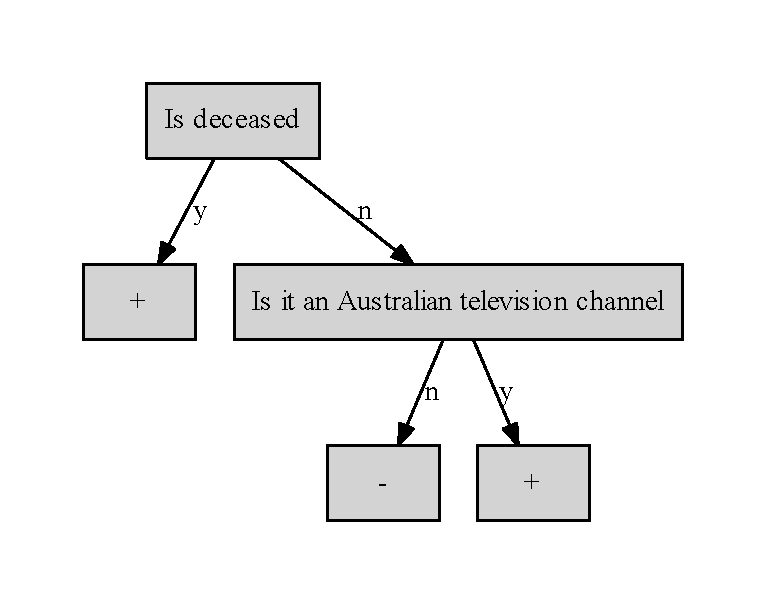
\includegraphics[width=0.6 \linewidth]{weird_trees.pdf}
%	\caption{A single level feature regarding things with a grammatical gender}
%	\label{fig:weird_trees}
%\end{figure}


%TODO: this is not great: too short, propo and upgrade should probably go to the new top part. this should be used to compare to specific papers as well
\section{Related Work}
One of the earliest methods of utilizing relational information is \emph{Inductive Logic Programming(ILP)} \cite{quinlan1990learning,muggleton1991inductive}, which induces a set of first-order formulae that define a good separation of the given training set.
Following this work, Relational Learning - techniques designed to utilize relational databases, have become increasingly prevalent. One such technique is that of View Learning \cite{davis2005view}, which generated new tables from existing ones, effectively performing feature generation for relational methods.
Unlike View Learning and other Relational Learning methods, our approach constructs a new learning problem in a different domain using the existing problem as a guide. Essentially,  we try to re-think our problem from a new direction, rather than trying to fit increasingly less connected entities to the original problem. Furthermore, the ability of our approach to locate locally beneficial features which may be difficult to otherwise detect is invaluable. Finally, we note that the use of decision trees during the feature generation process allows for a natural method by which to filter out features even before applying traditional feature selection mechanisms.

One major attempt at adding relational knowledge to traditional induction algorithms was \emph{propositionalization} \cite{kramer2000bottom}, which allows an unsupervised creations of first-order predicates which can then be used as features for propositional methods. A major setback of this process is that it generates an impractically large number of features, most of which irrelevant.  To this end, \emph{upgrade} methods such as ICL \cite{van2001upgrade} and SGLR \cite{popescul200716} were suggested, where instead of creating predicates a-priori, feature generation is performed during the training phase, in a more structured manner. While upgrade approaches bear some similarities to our approach, there are several critical differences, the key of which is the ability to more easily locate complex features through the use of existing induction algorithms.
We can see the Shallow feature generation algorithm (section \ref{shallow_section}) as a propositionalization algorithm using external knowledge as relational data.

Recently, there has been a strong trend of utilizing \emph{Deep Learning} \cite{lecun1998gradient,bengio2009learning} as a feature generation technique. Good examples of this can be seen in FEX \cite{plotz2011featurefull} and DBN2 \cite{kim2013deepfull}. These methods essentially form combinations and transformations on pre-defined features in a semi-supervised manner, thus yielding new, more predictive features. Our approach can be seen as a variation on the same concept, with the transformations being the construction of recursive learning problems, and the combinations being the classifiers constructed in the new problem domain. Our approach differs from those rooted in Deep Learning in both the use of external knowledge to enrich the feature space, and in that we allow more complex combinations in general, as deep learning approaches utilize weighted threshold functions, whereas our approach allows for generic induction algorithms.



\section{Conclusions}
%finishing up and summary

We presented a novel new approach to feature generation using relational data, based on constructing and solving new learning problems in the relational domain. 
Our feature generation algorithm constructs powerful and complex features, and can identify locally useful features as well as general trends. These features can be used along any traditional machine learning algorithm.
While we focused on applying this approach to text categorization problems, it is important to note that it is applicable to any classification problem where feature values are categorical and have semantic meanings, such as drug names, cities and so on. Although there is no simple way to generalize this approach to numeric features, we believe there are numerous domains where feature values do have semantic meaning, even excluding text-based domains.
While our approach only generates binary features, aggregation based techniques such as those used in SGLR apply here as well. We furthermore note that when solving non-binary classification problems, we can construct categorical features with, at most, the same amount of values as there are labels in the dataset.

A major source for potential improvement is the subject of matching values to semantic objects. Given the major advances in the field of Wikification \cite{bunescu2006using} in general and Entity Linking \cite{rao2013entity} in particular, these approaches can be used to link the initial text to entities within the semantic data without losing information, which may lead to better results, especially for text classification problems. We have seen in our experiments that primitive entity matching techniques may lead to mistakes which can cascade into poor features.

Another major potential avenue for improvement is to use the labelling techniques discussed section \ref{algorithm_section} as a way to directly label entities within the semantic graph, which yields a Collective Classification \cite{kajdanowicz2013collective} problem in the semantic domain. Solving this learning problem in turn allows us to label any entity within the semantic net, essentially yielding a labelled semantic net trained on our problem. We can then use this net to label new objects within the original problem context through a combination of entity extraction, usage of the semantic labels and label consolidation techniques.

%\clearpage
\vskip 0.2in
\bibliographystyle{theapa}
\bibliography{document}
%\bibliographystyle{plainnat}
%\bibliography{document}

\end{document} 